\chapter{Literature review}
\label{chp:2}

\graphicspath{{chapter_2/figures/}} % path to the figures folder of this chapter

%\dropcap{I}{n} our research group we do not publish literature review articles, and it will be difficult to convince me to change this policy\footnote{You can always try!}. We publish original research. This has consequences for this chapter of your thesis:

%\begin{itemize}
%	\item Keep it short. My suggestion\footnote{As with everything I write here (or say...): use your judgment! Sometimes there are good reasons for having even shorter or longer literature reviews.}: approximately 10 to 20 pages. 
%	\item Include lots of \textbf{relevant} references \cite{bessa2017a,bessa2018a} and briefly summarize the work.
%	\item In general, do \textbf{not} include the details of the articles you cite. Some articles can (and should) be described in more detail, but only when they introduce essential knowledge to understand your work.
%	\item Usually, an article can be summarized in one (or a few) sentences. Remember, the reader can always go to the original articles to understand the details of \emph{someone else's} work! 
%\end{itemize}	

%This policy has a couple of consequences:

%\begin{enumerate}
%	\item Your first paper will not be as easy as a literature review (sorry!)
%	\item You cannot use a large literature review as a scapegoat for not being original ;)
%\end{enumerate}	

%Note that this does not mean that a literature review is not important. On the contrary, {\color{red}knowing the literature well is usually the first step for good research}. It is important for you to \textbf{know} the research well, but you do not need to teach the reader about past research. You just need to \textbf{guide} him/her through that maze in a coherent and helpful way...

\section{Fused Filament Fabrication}
    \label{Fused Filament Fabrication}

To get a good understanding of the mechanical properties of Fused Filament Fabricated (FFF) produced parts, it is fundamental to have a good insight in the FFF process. Since this is a method that has been evolving quite extensively in the last decades, a quick review of the history and the process are presented in the next sections. 

\subsection{History}
    \label{History}
The FFF process has its fundamentals in polymer extrusion, which is a well known process well before the first 3D printer. Generally it is assumed that the first working robotic FFF 3D printer (as we know them) was developed in 1984, since that moment it has been a tool for manufacturing and prototyping that gained popularity in the next decades. 

%It was not until late 2000's that "desktop printers" (small affordable printers that could be used by particular users) were readily available to the public. In 1989 the founders of the currently leading 3D printer manufacturer "Stratasys" patented the Fused Deposition Modeling technology, also known as Fused Filament Fabrication (FFF). In 2005 some key patents expired and the technology became available to the public, this gave rise to a massive innovation movement called RepRap where different small businesses and individuals collaborated to design and optimize consumer focused FFF 3D printers.Different individuals even gained initial funding from different Research Councils. 
During the decade of 2010, 3D printing technology experienced an explosive growth. A wide variety of start-ups presented their systems on the market, with the consequence of being bought by big players like Stratasys \cite{Kamran2016ATechnology}. With these innovations also the process and products of 3D printers have been significantly optimized. From producing mostly fixtures, jigs, consumer, aesthetic and prototyping products, FFF parts are increasingly implemented as functional parts in e.g. machinery and vehicles. However, the mechanical properties are still a fraction of the conventional made counterparts and are unpredictable. To overcome this problem more research is being done in the process and properties of FFF products. Also new solutions such as reinforced polymers are being presented to create better functional parts. 
\clearpage

\subsection{Process \& hardware}
    \label{Hardware}
The basics of FFF have been  similar since the start of the technology, a polymer filament of a few millimeters in diameter (currently 1.75 and 2.85mm are most common) is pushed through a metal heating element before being deposited by a nozzle (a diameter of 0.4mm is most common, larger and smaller nozzles are also available). One resulting bead is defined as a "road". The nozzle and heating element assembly is also referred as the "hot end", depicted as "liquifier" in figure \ref{fig:Wirefeed}. For simplification the "extruder" is defined as the whole assembly of the mechanism for extruding filament, shown in figure \ref{fig:Wirefeed}. This hot end is attached to a moving mechanism that can have different principles of motion, most of the systems use stepper motors that are connected to the extruder trough rubber belts. This part is also referred to as "toolhead". These systems use three stepper motors which control the extruder in three degrees of freedom x, y and z directions in Cartesian coordinates. Alternatively, an axis of motion can be used to move the buildplate vertically or horizontally. Above mentioned systems are called "Cartasian printers". 

Another popular extruder positioning method is through 3 motors connected to worm wheels in vertical moving direction, with an arm connected to the extruder allowing it to also have three degrees of freedom, these systems are called "Delta-style printers". 

\begin{figure}[H]
    \centering
    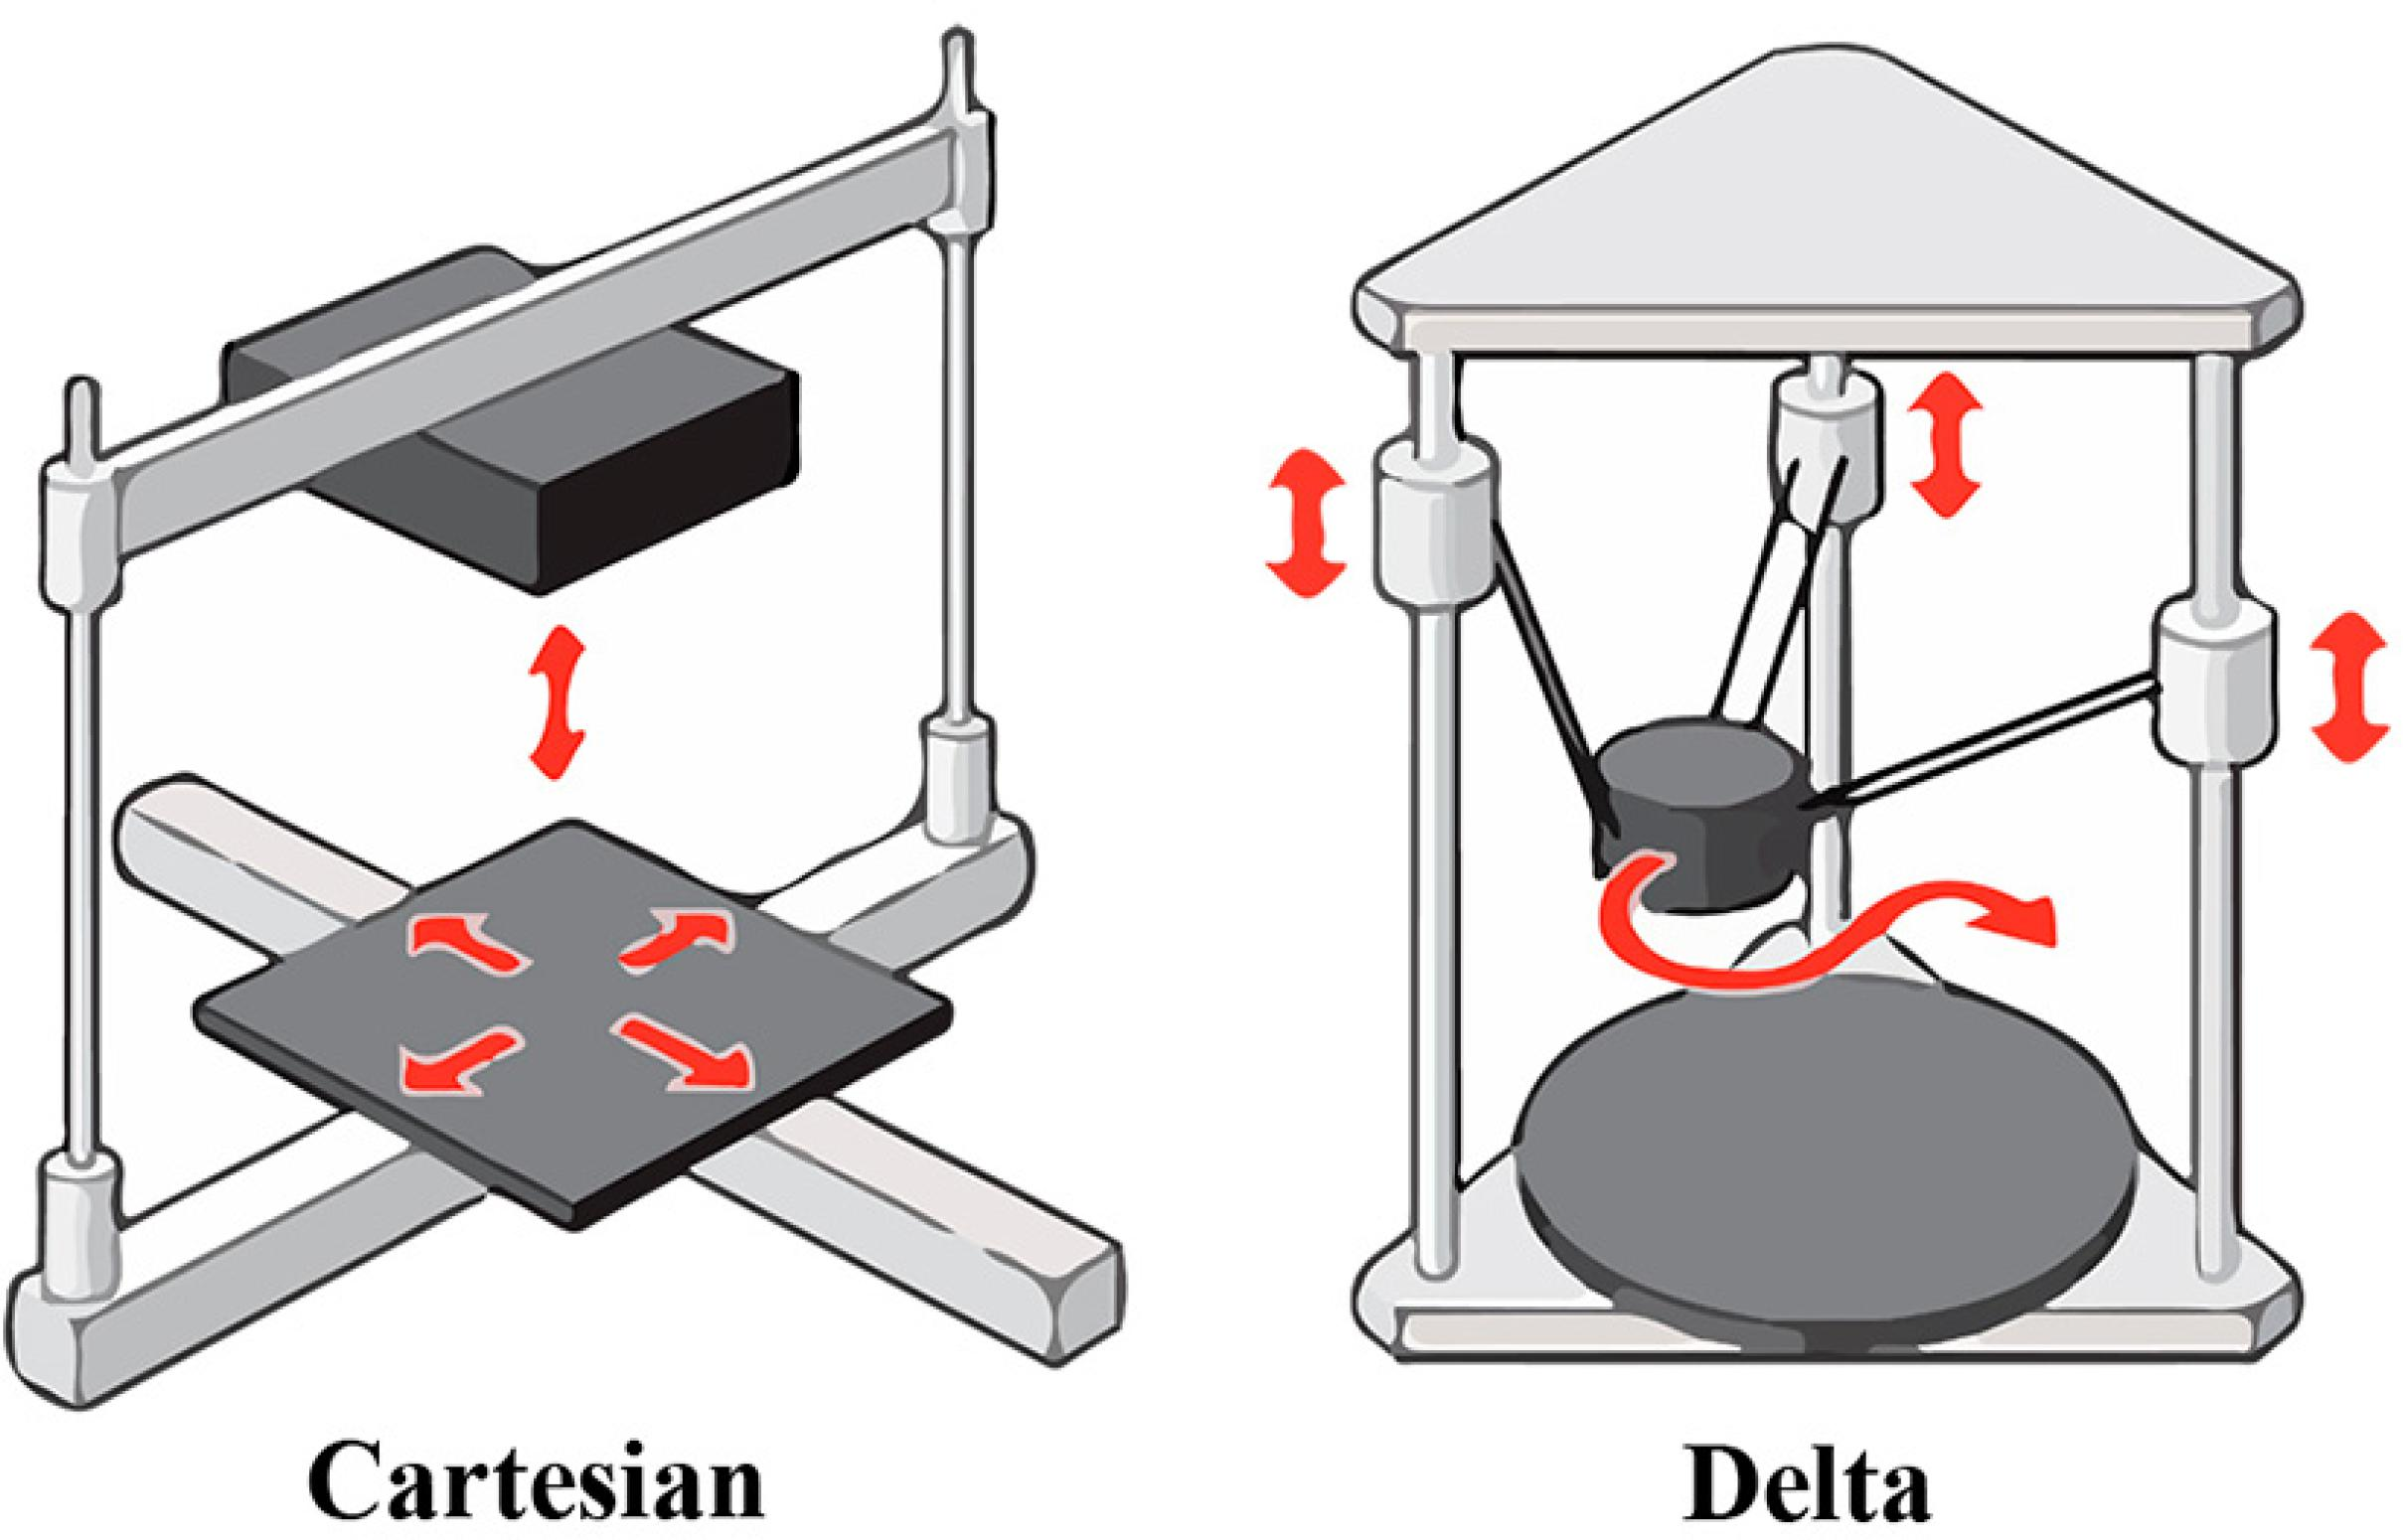
\includegraphics[width=0.40\textwidth]{chapter_2/figures/cartesiandelta.jpg}
    \caption{Comparison cartesian and delta system \cite{Turner2014AModeling}}
    \label{fig:cartesiandelta}
\end{figure}

In this thesis, the focus will be on cartesian style printers, the specific system that will be used for investigation is the Ultimaker S5 system \cite{Ultimaker2019UltimakerSheet} shown in figure \ref{fig:Ultimaker}. The exturder is positioned through a machine code named g-code above the so called "printbed", "builplate" or "buildplatform" and deposits molten filament in a particular path along the x-y plane. After finishing the programmed path of a supposed "layer" the extruder moves up in the z direction to start depositing a new layer on top of the previous one. The part can be removed with little to no effort from the buildplate. The buildplate has often an implemented heating element to prevent large temperature gradients in the first layers, which can result in so called warping (due to difference in shrinkage in layers the corners of the part can start to curl, resulting in de-lamination from the buildplate), this is often an issue with materials with a high glass transition temperature and thermal expansion coefficients \cite{Turner2014AModeling}. 

\begin{figure}[H]
    \centering
    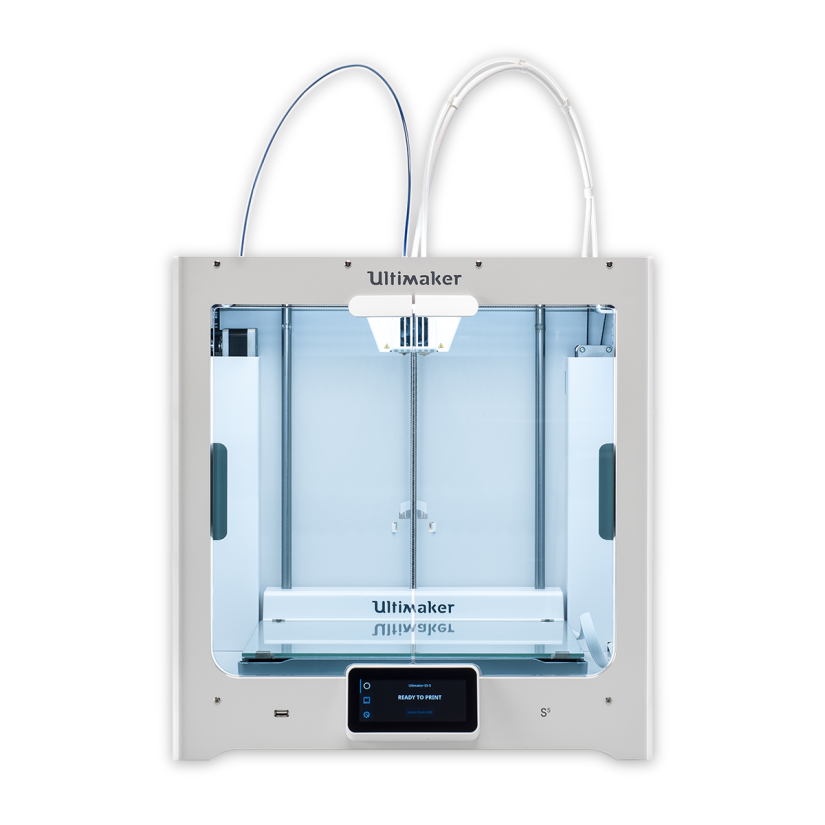
\includegraphics[width=0.40\textwidth]{chapter_2/figures/UltimakerS5.png}
    \caption{Ultimaker S5 \cite{Ultimaker2019UltimakerSheet}}
    \label{fig:Ultimaker}
\end{figure}

Turner et al.\cite{Turner2014AModeling} have clarified the process and the effect it has on the product, the relevant concepts will be presented here. Note that this system is typical for consumer based FFF systems and is (generally) the basis for more advanced systems. It might happen that systems use different processes, for this thesis the process of the Ultimaker S5 is assumed. 

\begin{figure}[H]
    \centering
    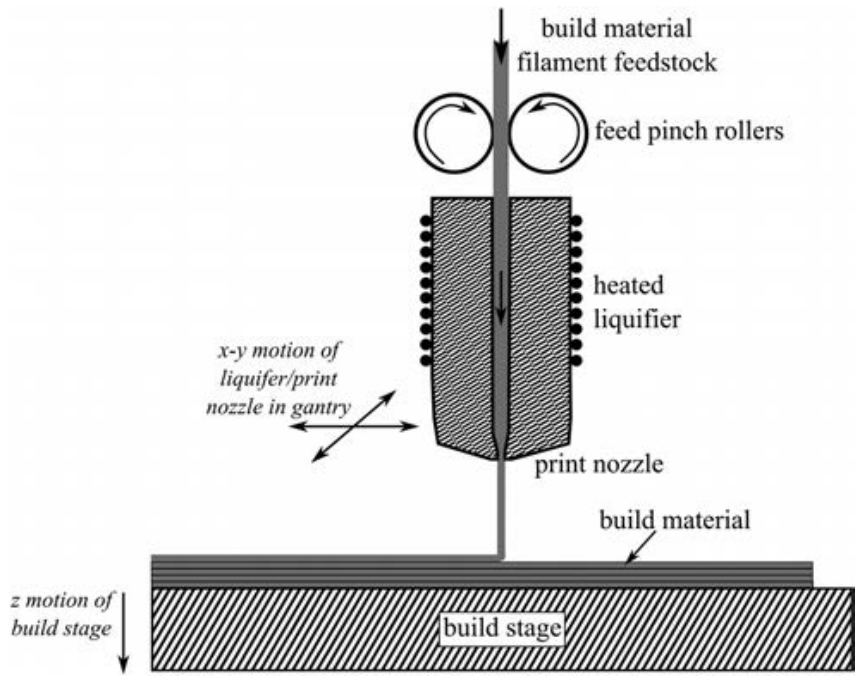
\includegraphics[width=0.50\textwidth]{chapter_2/figures/Wirefeedmechanism.PNG}
    \caption{Wire feed mechanism \cite{Turner2014AModeling}.}
    \label{fig:Wirefeed}
\end{figure}

\subsubsection{Feed mechanism}
    \label{Feed mechanism}
The feed mechanism is the root of the material supply, between two feed pitch rollers a filament of material is being pushed through a nozzle as can be seen in figure \ref{fig:Wirefeed}. The filament can be stored in a sealed container to prevent water absorption. Some materials are more prone to hygroscopy (like Nylon 66 and PLA), which during the extrusion results in the evaporation of the water and consequently in morphological changes in the material, blockages of the nozzle and formation of bubbles and porosity. This can be one of the issues of decreased mechanical properties, and should therefore be avoided. 

\subsubsection{Liquifier}
    \label{Liquifier}
The liquifier (figure \ref{fig:Wirefeed}) has a critical function: the softening of the polymer feed stock. This metal block has integrated heating elements to maintain a uniform temperature for liquefying the material.  A range of amorphous and semi-crystalline thermoplastic polymers (including fibers) with different melting and glass transition temperatures can be used in filament form as feedstock material. The liquifier temperature does normally not exceed 280$^{\circ}$C for consumer based systems, which excludes engineering polymers from use. It should be noted that due to the pressure and the shear force involved in the extrusion of filament through the nozzle, the polymer chains are being aligned in the direction of deposition (figure \ref{fig:polymerallignment}, which can have a significant impact on the mechanical properties of the part \cite{Mcilroy2017DisentanglementManufacturing}.

\begin{figure}[H]
    \centering
    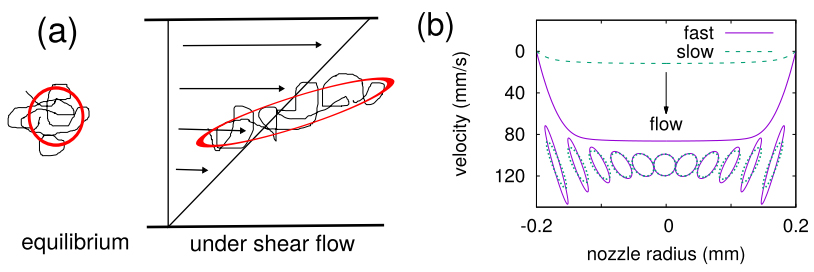
\includegraphics[width=0.6\textwidth]{chapter_2/figures/polymerallignment.jpg}
    \caption{a)Allignment of Polymer chains b)Velocity profile of polymer chains exiting the nozzle\cite{Mcilroy2017DisentanglementManufacturing}}
    \label{fig:polymerallignment}
\end{figure}

\subsubsection{Road deposition}
    \label{Road deposition}
The nozzle pushes hot filament onto the buildplate. During the extrusion the polymer melt is under stress, which reduces its volume due to deformation of energy being stored elastically. The nozzle hovers above the substrate at the prescribed layer height (often between 0.1 and 0.4mm), as can be seen in figure \ref{fig:Roaddepostion}. Consequently, the polymer melt is pushed outside and expands due to the absence of pressure. This phenomenon is called "dye swelling" and can be seen in figure \ref{fig:dieswelling}. Dye swelling plays a large role in the determination of the tolerance and surface roughness of a part. A ratio $(s)$ can be assigned to the swelling of the material with respect to the diameter of the die opening (nozzle). This value depends on the geometry of the nozzle, material properties (such as thermal expansion coefficient) and is generally in the range of 1.05 to 1.3. Shofner et al\cite{Turner2014AModeling} have found that the implementation of inelastic particles, such as short carbon fibers, have a positive effect of reducing the dye swelling, resulting in smoother surfaces (which is confirmed in empirical test with onyx, a carbon fibre filled nylon polymer. 


\begin{figure}
\centering
\begin{minipage}{.5\textwidth}
  \centering
    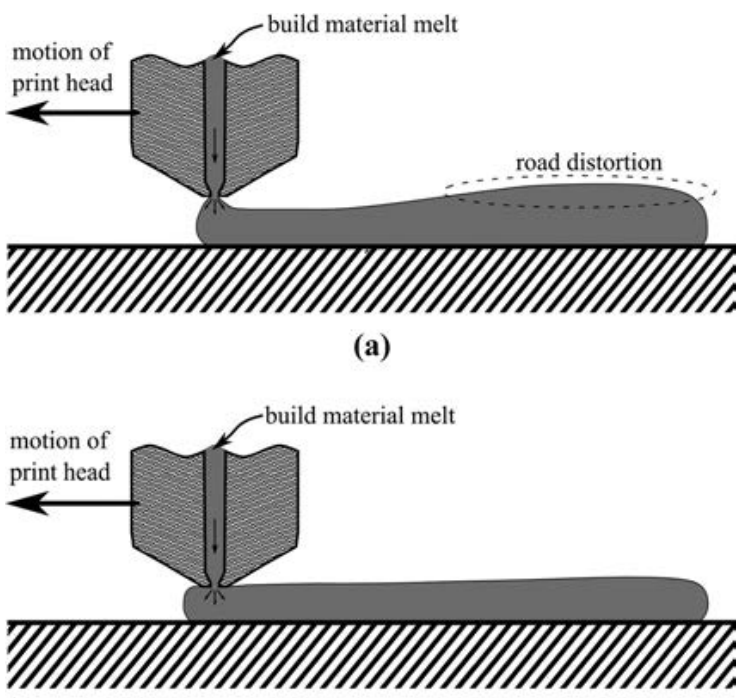
\includegraphics[width=.6\textwidth]{chapter_2/figures/Extrusion.PNG}
   \caption{Road deposition \cite{Turner2014AModeling}}
    \label{fig:Roaddepostion}
\end{minipage}%
\begin{minipage}{.5\textwidth}
  \centering
  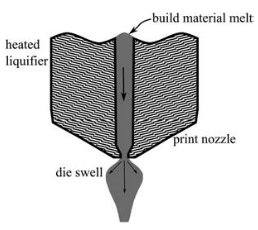
\includegraphics[width=.6\textwidth]{chapter_2/figures/dieswelling.PNG}
    \caption{Die swelling \cite{Turner2014AModeling}}
    \label{fig:dieswelling}
\end{minipage}
\end{figure}

The so called "bead" or "road" is deposited in an oblong shape (similar to a stadium shaped oval), and starts to cool due to convective cooling once it comes in contact with air and conductive cooling once it comes in contact with neighbouring roads. Bellini et al. \cite{Bellini2003MechanicalModeling} modelled this convective cooling assuming a heat transfer coefficient of $h =20 W/m^2$. In chapter 4 further investigation will be conducted on the shape of the road. Interestingly enough, the thermal conductivity of the feedstock material has a positive effect on the temperature of the bead after deposition. Instead of losing heat due to high thermal conduction, materials with high conductivity can more easily extract heat from the hot end at a larger distance, therefore creating better bonding between layers. 

\begin{figure}[H]
    \centering
    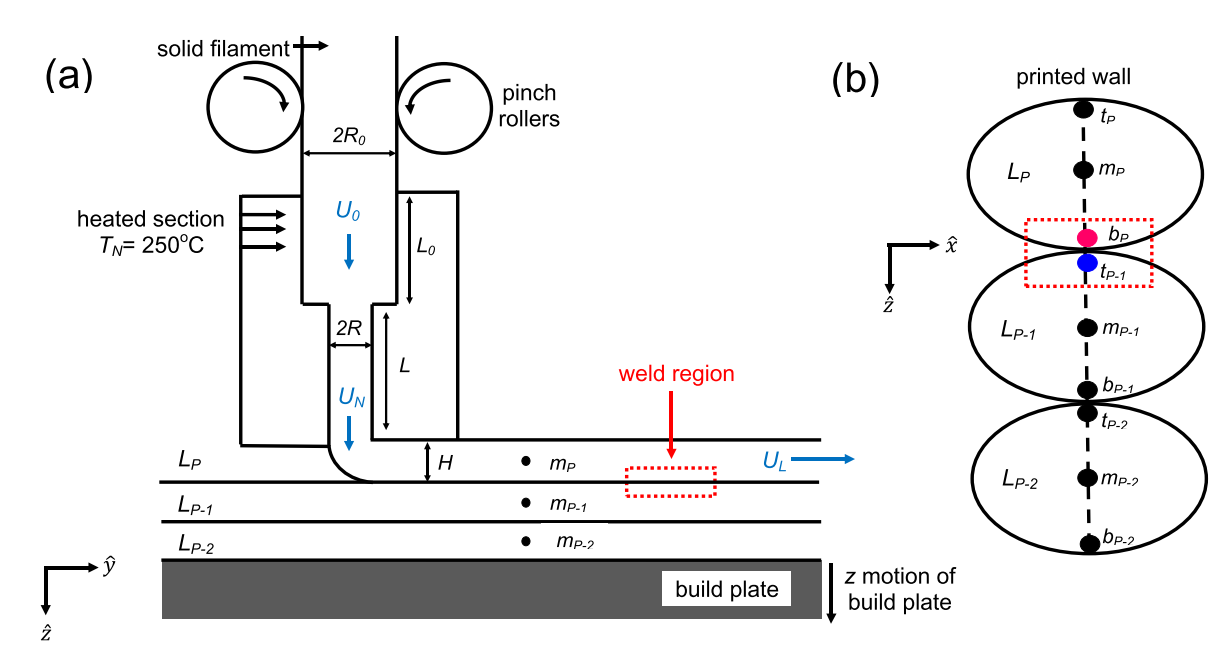
\includegraphics[width=0.7\textwidth]{chapter_2/figures/welding.png}
    \caption{a)Welding of subsequent roads. b)Heated top layer contacts with cooled lower layer \cite{McIlroy2017DeformationManufacturing}
    \label{fig:welding}}
\end{figure}

The touching surfaces of the roads are "welded" together if the temperature of both roads is high enough (figure \ref{fig:welding}). The deposited filament is practically uniformly melted, since the liquifier temperature is set at a higher temperature than the melting temperature ($T_m$) or glass transposition temperature for thermoplastics ($T_g$). For perfect bonding the surface of the lower road should also reach this temperature and maintain this for enough time. However, the temperature of the lower road has cooled since it was deposited. The strength of the bond is therefore a function of time and temperature of both roads and can be expressed in two different mechanisms: wetting and healing (figure \ref{fig:polymerwelding}). This is an anisothermal process of heating and cooling different layers at high rates as can be seen in figure \ref{fig:temperaturehistory}. One of the first researchers that began investigating this process where Thomas and Rodriguez \cite{Thomas2000ModelingRoads} followed by Bellehumeur et al.\cite{Bellehumeur2004ModelingProcess}and  Sun et al. \cite{Sun2008}. Seppala et al. \cite{Seppala2017WeldManufacturing} did an extensive study on the temperature profile of extruded roads and the bond forming after different layers are being deposited on top of it. The temperature history can either empirically be observed with an infrared camera, or can numerically be approximated when the toolpath of the extruder is known.There are currently software tools available which will generate a predicted temperature profile for specific layers in a particular FFF produced geometry\cite{Digimat-AM}. 

\begin{figure}[H]
    \centering
    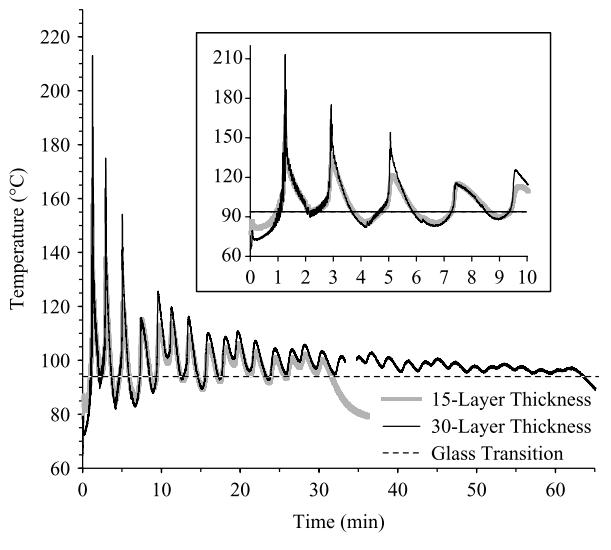
\includegraphics[width=0.4\textwidth]{chapter_2/figures/temperaturehistory.PNG}
    \caption{Temperature profile of the bottom filament \cite{Sun2008}
    \label{fig:temperaturehistory}}
\end{figure}

Wetting is defined by Wool \cite{WoolStrenghtInterfaces} as close molecular contact (van der Waals bonds) when two pieces of molten polymers are brought into contact followed by inter diffusion of chain segments back and forth across the wetted interface. The diffusion of polymer chains is called healing, which is investigated by Sun et al \cite{Sun2008}. After wetting of the roads, neck growth occurs which widens the area between adjunct roads. These three processes can be seen in figure \ref{fig:polymerwelding}. 

\begin{figure}[H]
    \centering
    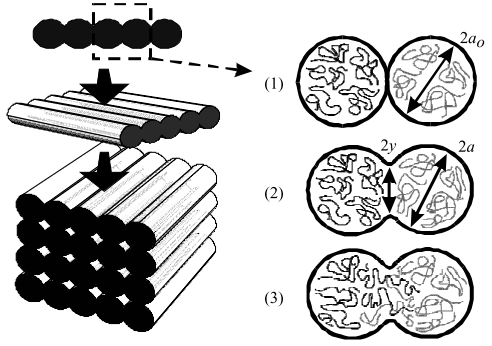
\includegraphics[width=0.4\textwidth]{chapter_2/figures/polymerwelding.PNG}
    \caption{Bond formation between roads: (1) contact, (2) wetting and necking (3) healing  \cite{Sun2008}}
    \label{fig:polymerwelding}
\end{figure}

After subsequent roads are deposited in layers on top of each other, a particular "mesostructure" of welded beads, with an elliptical shape, will appear. These mesostructures (shown in figure \ref{fig:mesostructure}) are analyzed in different articles \cite{Somireddy2017MechanicalMesostructure}
\cite{Somireddy2018DevelopmentFDM}
\cite{Li2002CompositeProperties} \cite{Rodriguez2001MechanicalInvestigation}
\cite{Rodriguez2003MechanicalModeling}
\cite{Blok2018AnComposites} 
\cite{Sun2008}, all conclude that the mesostructre has significant impact on the mechanical properties.
Most of the researchers used microtoming and optical microscopy to produce clear images (in the range of tenths of millimeters) of the mesostructure. These voids form a significant amount of porosity which has an adverse effect on the mechanical properties, resulting in stress concentrations and leading to premature brittle failure  near the porous region.  What is not observable in the mesostructure is the degree of healing between the roads. 
The majority of above mentioned researchers do not provide satisfactory information regarding their process settings or hardware used. Early experiments often incorporated Stratasys systems with their own produced ABS P400, due to their early market share. 

The final shape of the road depends on the surface tension, feed rate, viscosity, rate of cooling and interaction with the print head. There have been attempts of modelling the shape and spreading of the roads without being successful. A model proposed in the work of Turner \cite{Turner2014AModeling} assumes full wetting but does not account for the change of viscosity. The result significantly differs from empirical observations. 

\begin{figure}[H]
    \centering
    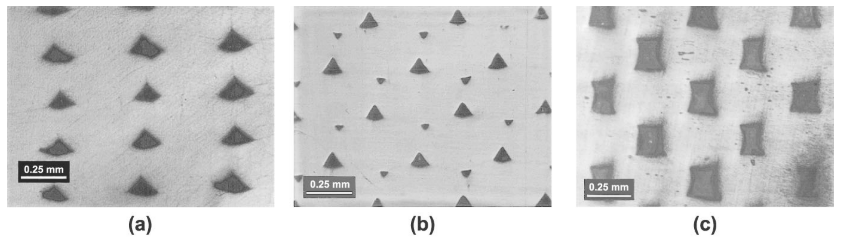
\includegraphics[width=1\textwidth]{chapter_2/figures/Mesostructure.PNG}
    \caption{Different types of mesostructures \cite{Rodriguez2001MechanicalInvestigation}}
    \label{fig:mesostructure}
\end{figure}

According to Sun, the amount of wetting and healing determines largely  the mechanical properties of the part \cite{Sun2008}. The healing of the polymer are related to the polymer material property called reptation time, which is the time a polymer needs, at a certain temperature, to "reptate" out of the other chains of the melt to acquire a new random position. Reptation is closely related to the glass transition temperature ($T_g$), the temperature where polymers start to diffuse and lose viscosity. After reaching this temperature polymer chains start to reptate exponentially faster. Different authors \cite{Mcilroy2017DisentanglementManufacturing}  \cite{Hart2018IncreasedAnnealing} \cite{Bartolai2016PredictingManufacturing} assume perfect bonding (full reptation) to be comparable to the mechanical properties of the middle of the road. With the help of WLF (Williams-Landel-Ferry graphs) a model can be made where reptation time is plotted as a function of temperature (figure \ref{fig:WLFreptation}). By producing a set of empirical data-points the WLF curve can be extrapolated \cite{Peterson2019ReviewPerspective}. With a higher temperature the amount of time needed for perfect healing is reduced, this can e.g. be achieved with a heated chamber or "envelope". According to Bartolai et al. \cite{Bartolai2016PredictingManufacturing} the strength of a road weld can be predicted using the following equation:

\begin{equation} \label{eq:weld}
\frac{\sigma_{weld}}{\sigma_{UTS}}=\left(\frac{t_{weld}}{t_{rep}}\right)^{1/4}
\end{equation}

In this equation $\sigma_{weld}$ is the weld strength in (MPa), $\sigma_{UTS}$ is the bulk ultimate tensile strength (in MPa), $t_{weld}$ is the time of molecular activity at a defined temperature (according to the WLF graph) at the interface (in seconds), and $t_{rep}$ is the time average reptation time of the polymer (in seconds). As $t_{weld}$ approaches $t_{rep}$ the polymer becomes fully healed and best strength is achieved. In the (limited) validation and verification of Bartolai, the conclusion was the of $\sigma_{weld}$ weld can be quite difficult for an accurate prediction.

\begin{figure}[H]
    \centering
    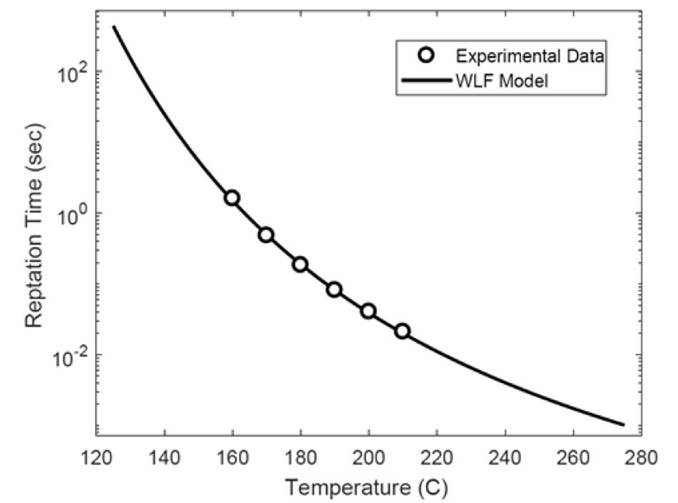
\includegraphics[width=0.4\textwidth]{chapter_2/figures/WLFreptation.PNG}
    \caption{WLF model, reptation time is a function of temperature \cite{Seppala2017WeldManufacturing}}
    \label{fig:WLFreptation}
\end{figure}

\subsubsection{Build plate and chamber}
    \label{Build plate and chamber}
The liquefied filament is deposited on the build plate (also called printbed) and is consequently deposited on top of the previous layers. The buildplate can be as simple as a piece of metal or glass. However, there are some crucial aspects concerning the properties of the bed. The adhesion of the first deposited layer with the bed is very important to prevent de-lamination during the process. Therefore, heat elements are used to decrease steep heat gradients in the part, which result in warping. To prevent the bed itself from deforming (as little as a few hundredth of a mm can have negative impact on the first layer) a material with a low thermal expansion coefficient is chosen (e.g. glass). The bed temperature has a positive effect on the layer bonding in the lower region of the part. However, this is only "felt" in roughly the first centimeters of the part trough conduction. It has been concluded that a higher overall temperature of the chamber has a beneficial impact on the road healing and subsequently on the mechanical properties\cite{VeenEnhancingTemperature}. More advanced systems therefore implement a heated envelope.

\subsection{Process parameters}
    \label{Process parameters}
Since the process parameters of the FFF process have major influence on the resulting parts, it is essential to analyze the parameters and identify their influence on the mechanical properties. In this section the important parameters are highlighted.

%part about slicers
Most of these setting are defined by the so called "slicer" software, which is used to edit setting before generating a machine code that can be read by the printer. Certain machines have unique compatibility with a certain slicer (e.g. Eiger software from Markforged), or are produced by a manufacturer which also allows compatibility with other FFF systems (e.g. Cura from Ultimaker) or are produced  by a third party software developer (e.g. Simplify 3D, Slic3r). These softwares have similar settings that can be adjusted which will result in a  trade-off between speed and weight versus resolution, precision and mechanical performance. Since this thesis is mostly based on an Ultimaker S5 system \cite{Ultimaker2019UltimakerSheet}, and Cura is used as its slicer by the manufacturers, the terminology and parameters of Cura will be used as a benchmark. 

The most significant parameters that have effect on the product are:\\
- Layer height (mm)\\
- line width (mm)\\
- Feed rate (mm$^3$/s)\\
- Extrusion temperature ($^{\circ}$C)\\
- Envelope temperature ($^{\circ}$C)\\
- Build plate temperature ($^{\circ}$C)\\
- Travel speed (mm/s)\\
- Infill density (\%)\\
- Infill orientation and shape ($\theta$)\\
- Airgap (mm)\\


Regular slicers use different type of settings for different elements in a part. Let's consider the cross section of a cube (as can be seen in figure \ref{fig:Shell}) for FFF printing. Once a CAD (computer aided design) file (often in the form of a STL "stereolithography" file) or other geometrical digital drawing supported by the slicer is uploaded, the slicer will define different settings for different elements. Most important being: Bottom layers, Outer shell (walls), top layers, infill. The effects of the  elements will be outside the scope of this thesis and can be easily found online (3Dhubs \cite{3DHubs2018OnlineQ4/2018}, All3D \cite{all3dpAll3dp}, Ultimaker \cite{UltimakerSpeed}, Simplify 3D\cite{Simplefy3DPrintGuide}). For this project the focus is on parts with only bottom-layers, mimicking fully "dense" parts. Applying only bottom layers will generate parts with best mechanical properties per volume.   \cite{Li2017TheProperties}

\begin{figure}[H]
    \centering
    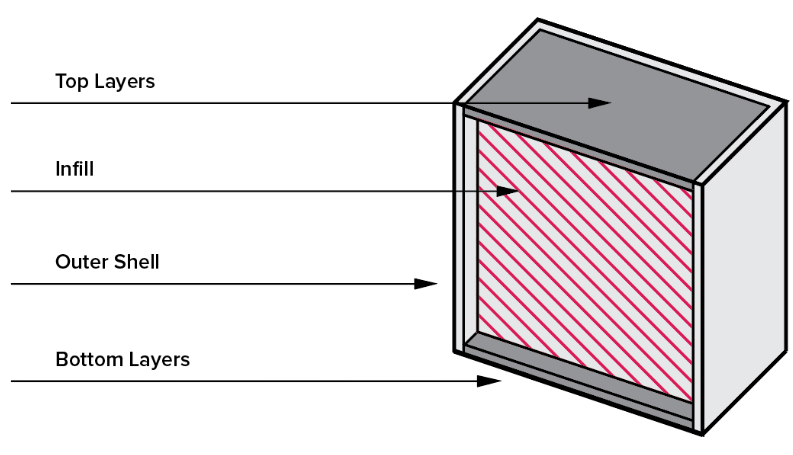
\includegraphics[width=0.5\textwidth]{chapter_2/figures/Shell.PNG}
    \caption{Elements of a 3D printed part \cite{Redwood2017TheApplications}}
    \label{fig:Shell}
\end{figure}
Effort that needs to be highlighted is the work of  Li et al. \cite{Li2017TheProperties} who generated empirical data and derived numerical models displaying the relation of temperature related parameters with the tensile strength of PLA, while maintaining other parameters constant.

According to parameters studied by Ahn et al. \cite{Ahn2002AnisotropicABS} the air gap and raster orientation are the parameters most significantly affecting the mechanical properties. This is explained by the fact that the air gap is directly linked with the porosity and the raster orientation is directly linked with the stress applied at the road interfaces.
A similar but more extensive research has been conducted by Mohamed et al. \cite{Mohamed2016EffectExperiment}, resulting in the same conclusion.

\subsubsection{Layer height}
The layer height is the height of one layer, subsequently also the height of one road. Increasing this parameter will decrease the print time proportionally, the drawback is higher surface roughness, larger porosity, larger stress concentration points and worse layer bonding. In Cura the layer height is limited between 0.04 and 0.32 mm. Since the polymer is welded by applying pressure and heat, different researchers assume that the roads have a horizontal and vertical overlap. This is about 10\% according to Somireddy \cite{Somireddy2017MechanicalMesostructure}.  The emperical results of Li et al. \cite{Li2017TheProperties} regarding the layer height parameter are shown in figure \ref{fig:Layerheigth}.

\begin{figure}[H]
    \centering
    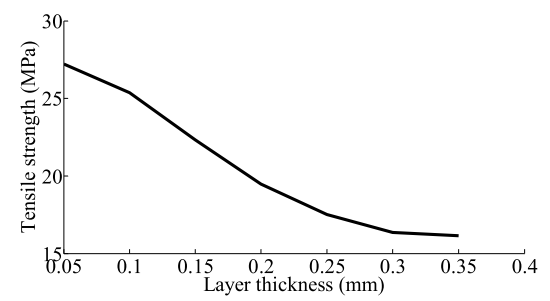
\includegraphics[width=0.5\textwidth]{chapter_2/figures/Layerheight.PNG}
    \caption{Layer height against tensile strength for XY[45/-45] samples \cite{Li2017TheProperties}}
    \label{fig:Layerheigth}
\end{figure}

Li \cite{Li2017TheProperties} explains that a smaller layer height will actually increase bonding between roads. High conductivity combined with the small volume that needs to be heated will positively affect the temperature history of the interface, compared to thicker layer heights where the heat flux is not able to heat the material as much as for the thinner counterparts. This is also confirmed by Kuznetsov \cite{Kuznetsov2018StrengthProcess}, who additionally claims that a reduced layer height also limits porosity in a part.

\subsubsection{Line width}
This process parameter can be misleading. According to Somireddy \cite{Somireddy2017MechanicalMesostructure} FFF systems produce roads that are set to have a 10\% overlap with its neighbouring roads in the xy plane. The line width defines the distance between adjacent roads, which could be assumed as nominal line width or the distance between roads. According to him the extruded line width is therefor about 10\% wider, if one would extrude a single road with a line width of 0.4 mm and a layer height of 0.2 mm it would be observed that a 10\% larger ellipse is produced. 
%By personal observation it was observed that multiple single roads deposited on top of each other produce a width that is 5-10\% larger than the nominal line width. 
This is in line with the observed increase in dimension for the production of fitted parts. A similar theory is proposed by Hodgson \cite{GaryHodgsonSlic3rMath}, "Extrusion Width is the thickness of a single filament extruded either in free air or above a surface. It's not the distance of two adjacent paths since some overlap will be generally applied in order to get better bonding."
When printing only bottom layers the roads are constrained by the substrate on the bottom, by the nozzle on the top, and possibly by a road on one side.  In figure \ref{fig:roadconnecting} the sintering of roads can be observed. The problem with this model is the fact that the overlapped material is not accounted for. In the chapter 4 a new model will be presented. There is currently not a consensus on the form of the mesostructure, this is partly due to large development and  variety of printers and available printer settings.

\begin{figure}[H]
    \centering
    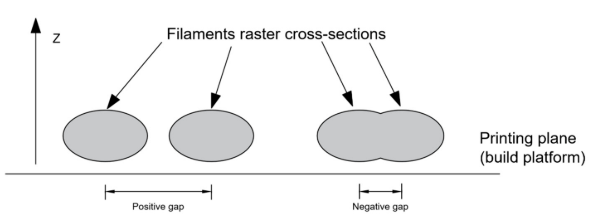
\includegraphics[width=0.7\textwidth]{chapter_2/figures/roadconnecting.PNG}
    \caption{A schematic representation of filament cross-sectional areas, showing the difference between positive and negative gaps \cite{Cuan-Urquizo2019CharacterizationApproaches}}
    \label{fig:roadconnecting}
\end{figure}

The range of the line width process parameter is limited by the nozzle diameter. For a nozzle of 0.4mm Cura allows for a line width ranging between 0.25 to 0.8. According to Montero \cite{Montero2001MaterialExperiments} a variation in line width has no significant effect on the mechanical properties of the part. Thomas \cite{Thomas2000ModelingRoads} and  Kuznetsov\cite{Kuznetsov2018StrengthProcess} notice a positive effect in inter-road bonding with increased line width.
%due to the larger  volume which cause prolongation of high temperature in the contact points and a reduction in porosity.  
%[for revision] The slicer always calculates the roads to be tangent, meaning that a 4mm wide beam will generate 10 0.4mm wide roads. Increasing this will have similar effects as increasing the layer height. This generates often just enough polymer to sinter the surfaces together, in comparison with the layer height, the different roads are not aided by gravity for better bonding. Be aware that the line width can also be influenced by inconsistencies of the filament. Filaments for the ultimaker have a nominal diameter of 2.85 +- 0.05, which mean that the road line width might have a fluctuation of 2\%.

\subsubsection{Airgap}
The airgap is defined as the gap in between different roads in the xy plane (intra-laminar) figure \ref{fig:roadconnecting}. Generating an airgap that is the same size of your road width will half your infill density, creating an negative airgap will produce an overlap between roads. It is not possible to select a negative value in Cura (implying an overlap of roads). This was possible in the Stratasys slicer settings, and has been thoroughly studied in different experiments \cite{Somireddy2017MechanicalMesostructure}  \cite{Rodriguez2001MechanicalInvestigation}   \cite{Ahn2002AnisotropicABS}  \cite{Dawoud2016MechanicalTechniques} \cite{Gebisa2018InvestigatingExperiment}
\cite{HossainImprovingParameters}
and resulted in higher density and mechanical properties (increase of about 5-10\% in $E_{11}$, $E_{22}$ and a 10\% increase in $G_{12}$) at the cost of speed and higher surface roughness and distortion. Additionally, the excess material can be accumulated on the nozzle and the part itself. Gebisa et al. \cite{Gebisa2018InvestigatingExperiment} claim that a negative airgap has also a negative influence on the heat transfer since the roads are deposited very close to each other and that more room facilitates the spread of semi-molten material between the gaps, resulting in structurally stronger parts. The conclusion of most experiments is that for ABS a negative airgap of not more than 10\% can lead to improvements in mechanical properties without significant influence on the dimensional accuracy and surface quality. It appears that  slicers have optimized this phenomena in the past years to achieve minimal porosity \cite{GaryHodgsonSlic3rMath}. Simplify 3D has the option to enhance the infill extrusion width for only the infill (Cura can only modify it for the whole part).
If we consider Somireddy's \cite{Somireddy2017MechanicalMesostructure} mesostructure images for regular settings a 10\% overlap is observed,  if the line width is reduced with 10\% while the extruded width remains equal,  approximately 20\%overlap is observed figure \ref{fig:Meso10&20}. The section \ref{mesostructure} will address this subject in more detail.
We can conclude from this analysis that negative airgap has an optimum where the mechanical properties are optimized without significantly distorting the surface of the product, it seems that this is already applied in some slicers. 

\begin{figure}[H]
    \centering
    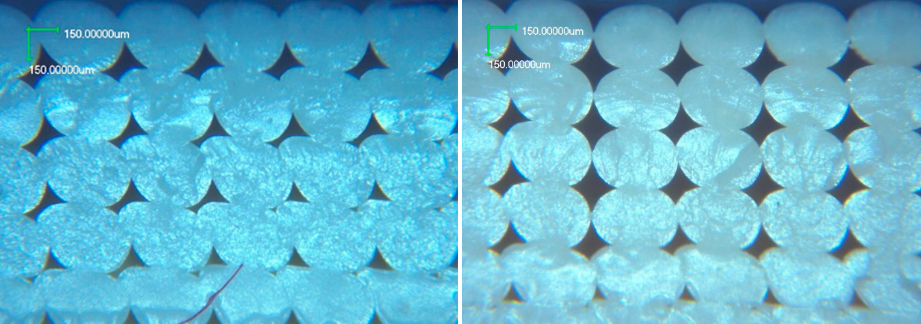
\includegraphics[width=0.8\textwidth]{chapter_2/figures/Meso10and20.jpg}
    \caption{Mesostructure with 20\% overlap (left) 10\% overlap (right)\cite{Somireddy2017MechanicalMesostructure}}
    \label{fig:Meso10&20}
\end{figure}

\subsubsection{Feed rate}
The feed rate is the volume of filament that is extruded per timescale. Since this is automatically calculated by Cura as a function of the layer height, line width and speed, it is difficult to precisely enhance, therefore it is defined as a multiplier of the default setting. Adjusting this will multiply the original calculated feed rate with a defined factor. This can for example fix under-extrusion (figure \ref{fig:underextrusion} when the feed rate is too low, resulting in bad bonding and large gaps) which is detrimental for the mechanical properties of the part. It can also compensate for over-extrusion \ref{fig:overextrusion}, which is detrimental for tolerance and accuracy. However, this could also be used to increase the extrusion to generate the so called "negative air gap". By increasing the flow multiplier, a wider road can be deposited without an increase in distance between roads as would happen with increase line width. This could be a detour to achieve the same increase in mechanical properties as a negative air gap would have.
We can conclude that the feed rate is closely related to the negative airgap parameter. The theory presented above and at the subsection of "line width" is supported by Patanwala et al. \cite{Patanwala2018TheComposites}, who wrote a detailed report on the characterization of the flow rate and bonding of carbon nanotubes-PLA composites.  
\begin{figure}
\centering
\begin{minipage}{.5\textwidth}
  \centering
    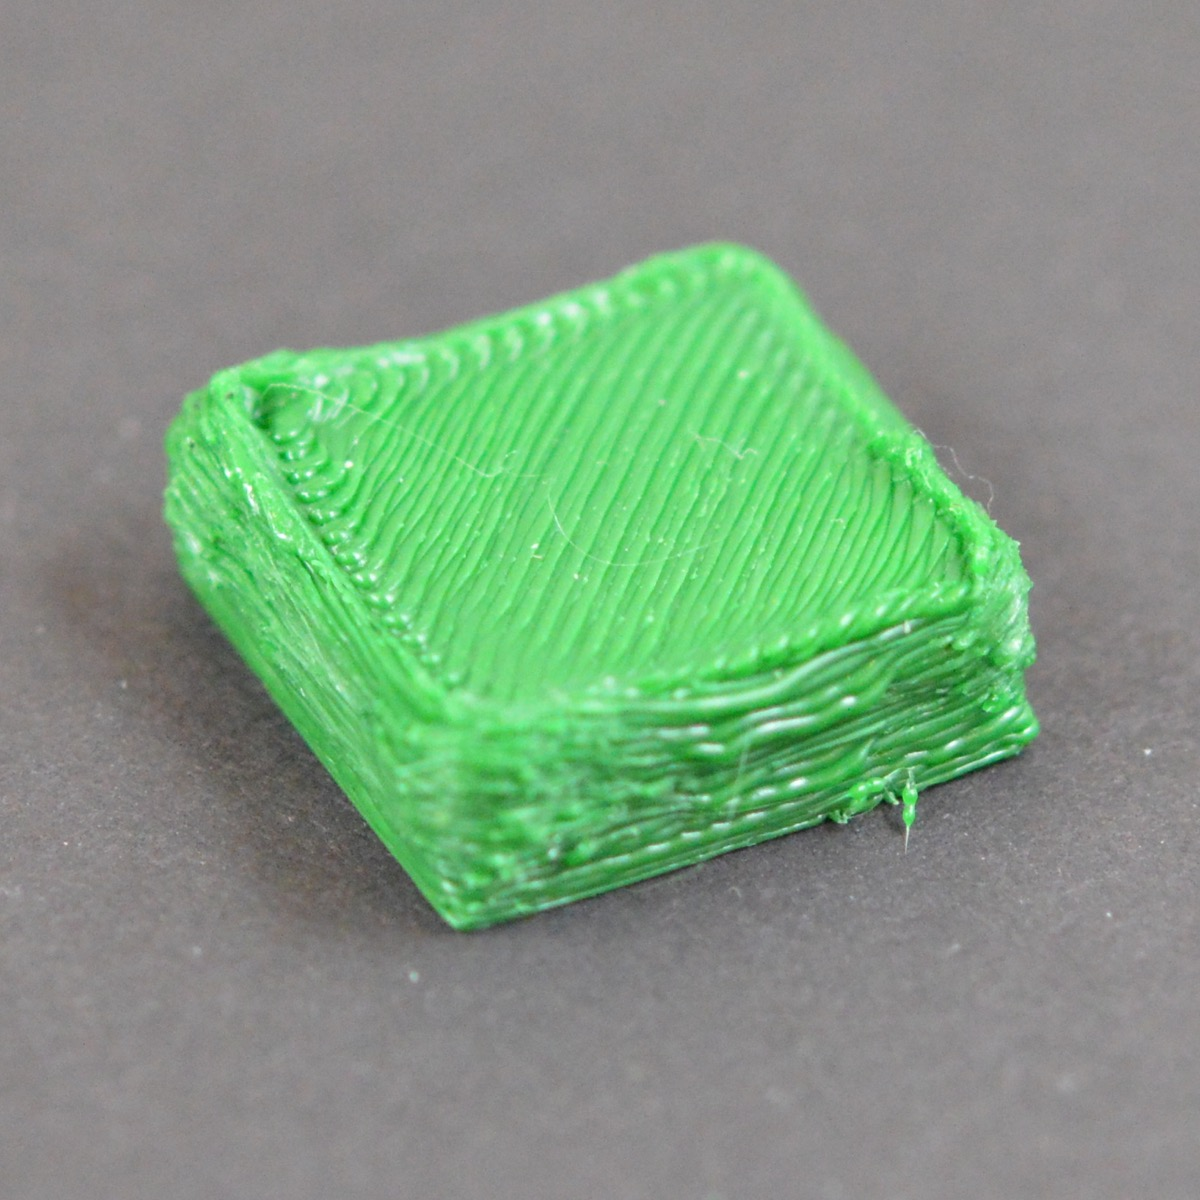
\includegraphics[width=0.5\textwidth]{chapter_2/figures/overextrusion.jpg}
    \caption{Overextrusion generating\\ 
    distortion of the part \cite{Simplefy3DPrintGuide}}
    \label{fig:overextrusion}
\end{minipage}%
\begin{minipage}{.5\textwidth}
  \centering
    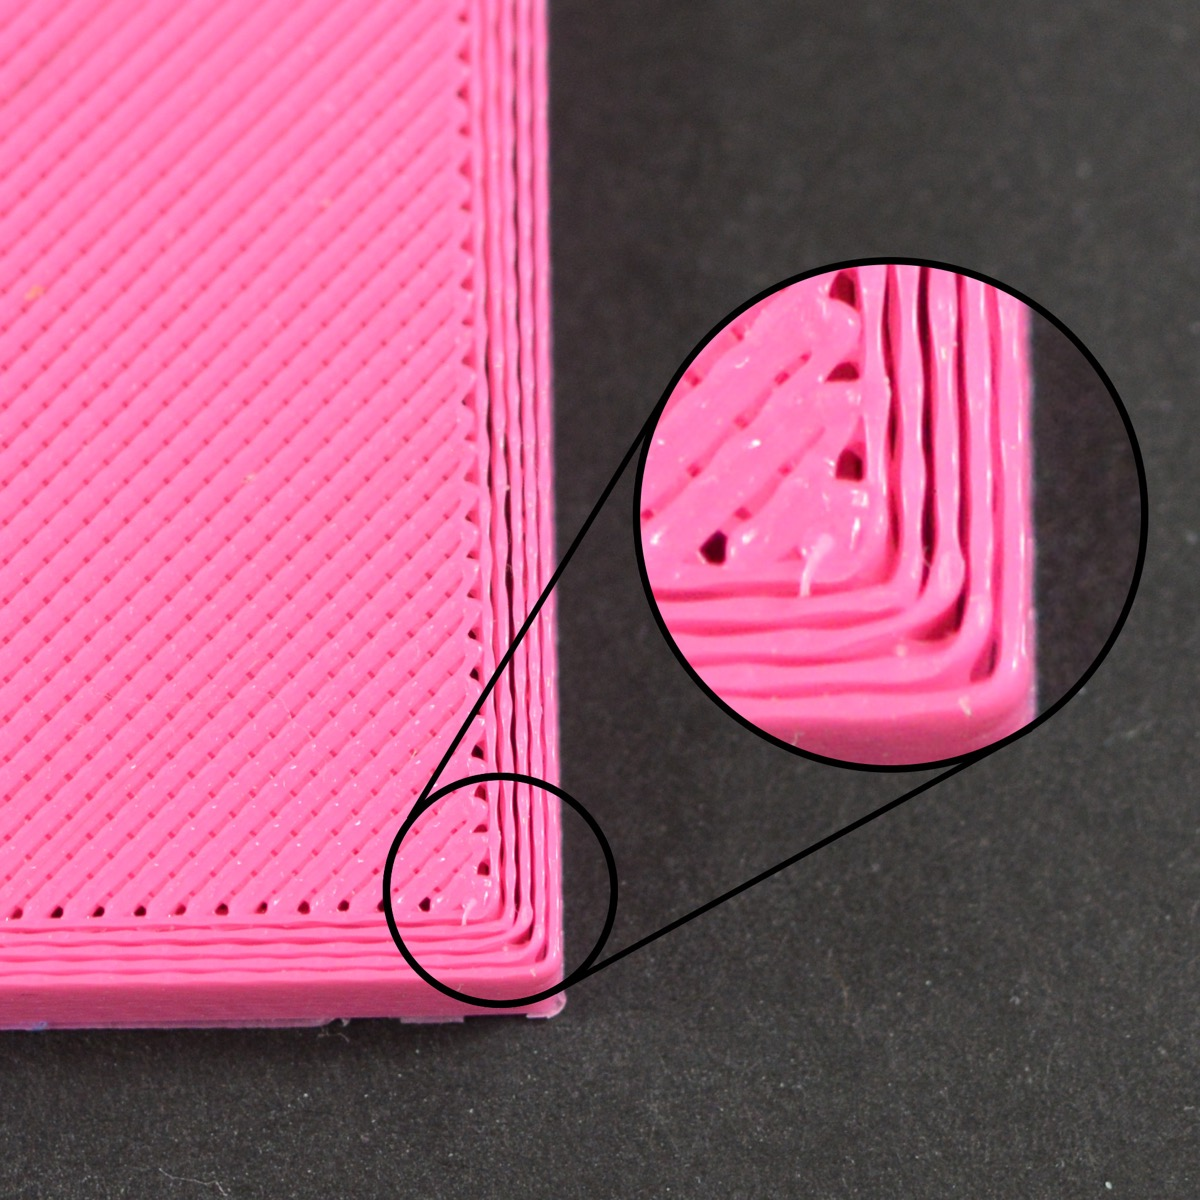
\includegraphics[width=0.5\textwidth]{chapter_2/figures/underextrusion.jpg}
    \caption{Underextrusion generating limited contact areas between roads \cite{Simplefy3DPrintGuide}}
    \label{fig:underextrusion}
\end{minipage}
\end{figure}

\subsubsection {Extrusion temperature }
The extrusion temperature is defined as the constant temperature of the extruder. This setting is different for every material. To make a material flow more the temperature can be increased, this can help for very fast prints, or in the case of under-extrusion. The dangers of printing too hot are, especially for small sections, a distortion of geometry due to a drop in viscosity. If the temperature is too low, the filament is too viscous to be extruded out of the nozzle, resulting in under extrusion or extrusion issues.  
There is an optimal range for the extrusion temperature which has been studied by Montero \cite{Montero2001MaterialExperiments} and others.
%as can be seen in figure \ref{fig:Montero}

\subsubsection {Envelope temperature }
Advanced FFF systems include a heated chamber or envelope. This is applied to increase the bonding of the roads, different studies \cite{Sun2008} \cite{Bellehumeur2004ModelingProcess} have shown that the bonding properties (healing and wetting) are affected by temperature and time. The downside is the possibility of small segments being heated too much, which results in distortion. The optimal envelope temperature for semi-crystalline materials is between $T_g$ and $T_m$. For amorphous polymers this is more problematic, since they do not have a specific melting temperature, instead they have a plateau after $T_g$ as can be seen in figure \ref{fig:EvsT}, the first observation would be to not exceed the temperature of this plateau.
According to van Veen \cite{Veen2019EnhancingTemperature} a clear relation was found between the envelope temperature and the bonding between layers, this is supported by the healing theory. 

\begin{figure}[H]
    \centering
    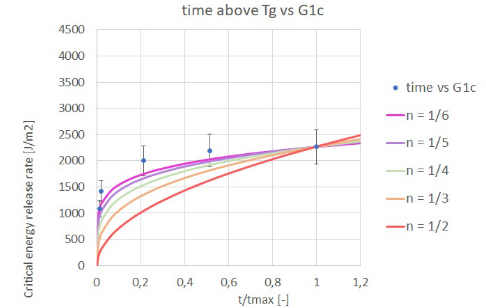
\includegraphics[width=0.5\textwidth]{chapter_2/figures/Dennisgraph.png}
    \caption{Critical release energy rate vs. the time parts spend above $T_g$\cite{Veen2019EnhancingTemperature}}
    \label{fig:Dennisgraph}
\end{figure}

\subsubsection {Build plate temperature }
The buildplate temperature is generally near the $T_g$ to limit thermal stresses and warping. As a beneficial side effect, it constantly heats up a set of layers touching the buildplate.
The quantitative effects of the build plate temperature on the mechanical properties of the part have not been studied yet. 
%possible conduction laws, predicting temperature??

\subsubsection {Print speed }
Print speed proportionally alters the process times,  but comes at a cost of larger in-homogeneity. Due to a large amount of accelerations the feed rate can differ trough-out the part. Often over-extrusion is observed near the walls of a layer.

A low speed (approximately 35 mm/s) should be used to avoid large speed differences \cite{Li2017TheProperties}.  In figure \ref{fig:speedgraph} the dependency of the speed related to the position is shown.

\begin{figure}[H]
    \centering
    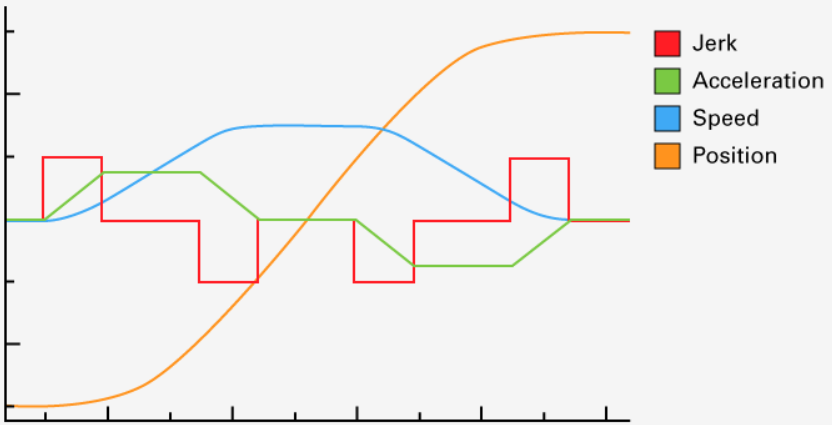
\includegraphics[width=0.4\textwidth]{chapter_2/figures/Speedgraph.PNG}
    \caption{Speed graph of the toolhead while printing \cite{UltimakerSpeed}}
    \label{fig:speedgraph}
\end{figure}

Li \cite{Li2017TheProperties} also investigated the effect of the deposition velocity on the tensile strength as can be seen in figure \ref{fig:depositionspeed}

\begin{figure}[H]
    \centering
    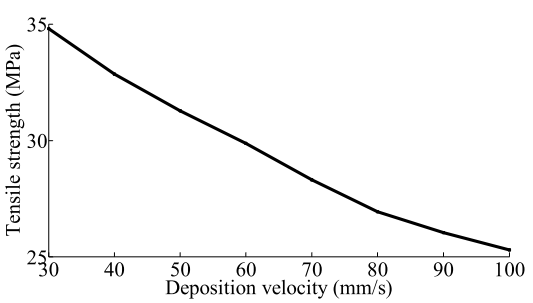
\includegraphics[width=0.5\textwidth]{chapter_2/figures/depostionspeed.PNG}
    \caption{Deposition velocity against tensile strength for XY[45/-45] samples \cite{Li2017TheProperties}}
    \label{fig:depositionspeed}
\end{figure}

Print speed directly influences the feed rate, which is most likely the cause of a decrease in mechanical properties with an increasing speed. Li also explains that for slower speeds the bottom layers remain at a temperature higher than $T_g$ for a longer period of time, which suggest that the adjacent filaments have more time to bond.

\subsubsection{Infill density}
The infill percentage determines the percentage of material with respect to air used in the infill structure. The infill is generally enclosed by so called wall layers (also called perimeters) and top and bottom layers. These roads form a solid shell on the surface. This volume of the infill can have different geometries, ranging from simple rectangles, to intricate 3D patterns as can be seen in figure \ref{fig:Infill}. The density can be changed in a variety of forms, creating thicker lines, more lines, direction etc. For this thesis the focus will be on structurally optimized parts, which includes 100\% infill (which won't result in a related relative density since there is a high amount of porosity).

\begin{figure}[H]
    \centering
    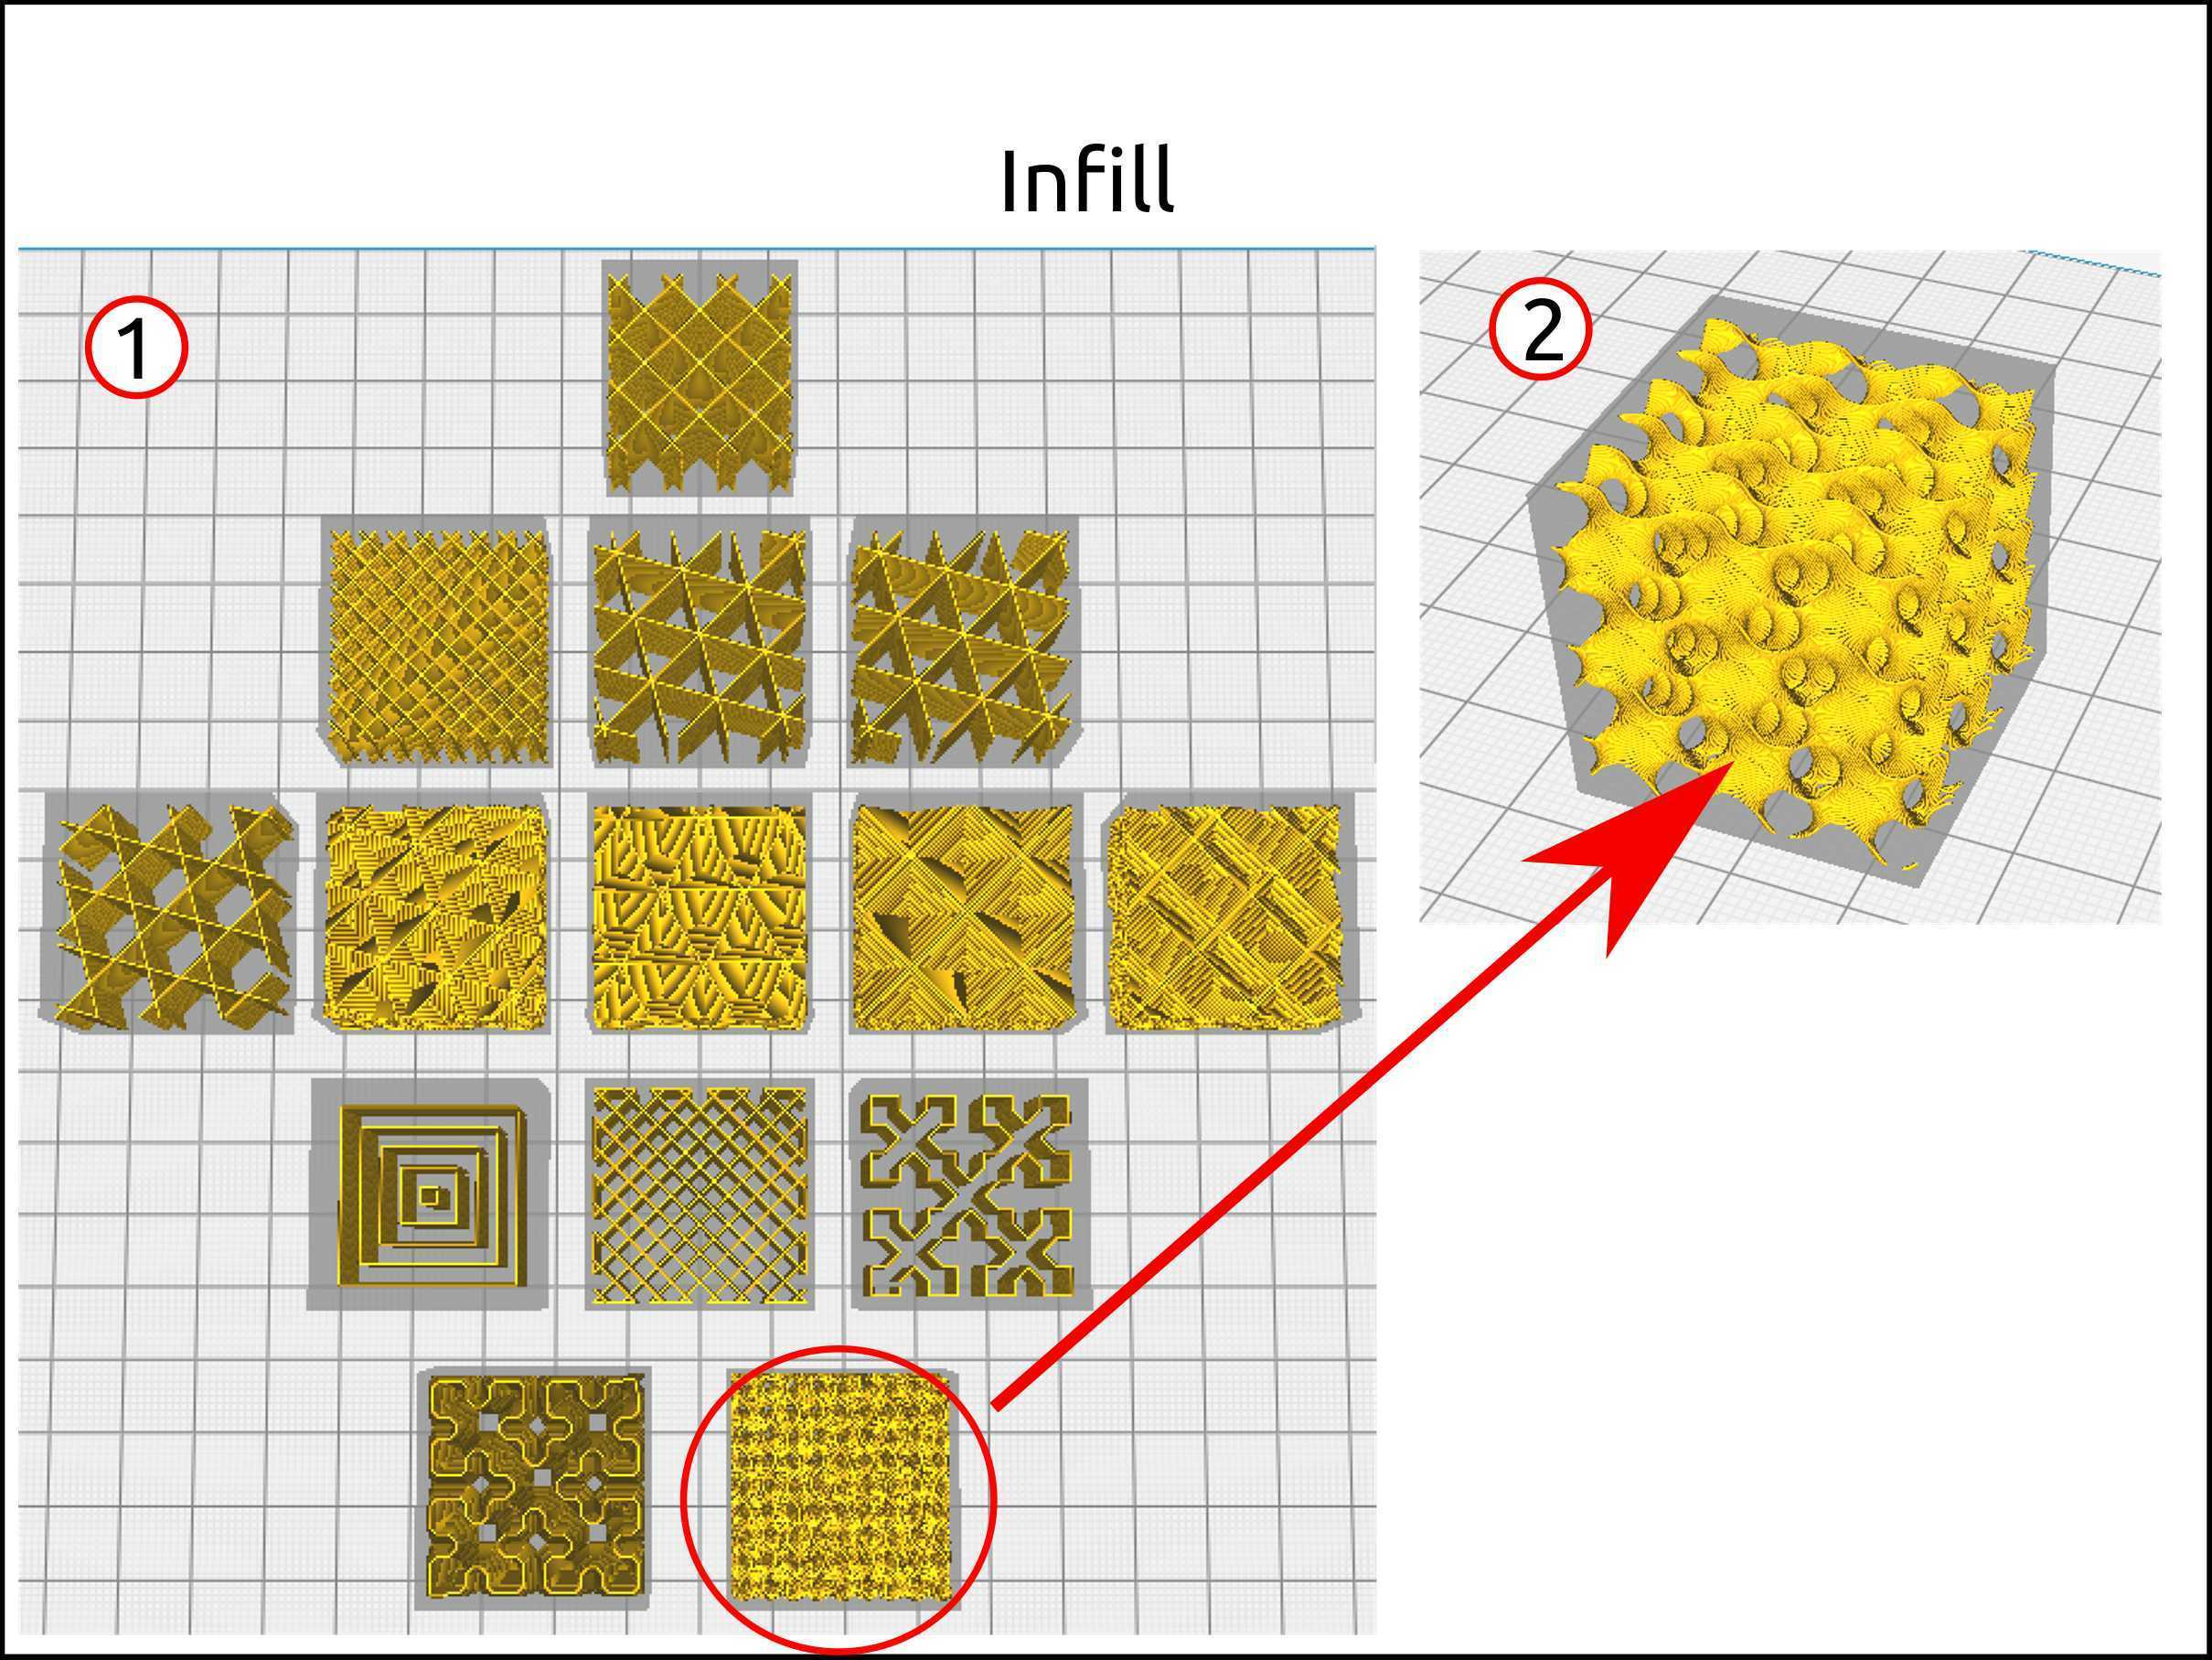
\includegraphics[width=0.5\textwidth]{chapter_2/figures/Infillbetter.jpg}
    \caption{Different types of infill \cite{UltimakerSpeed}}
    \label{fig:Infill}
\end{figure}

\subsubsection{Road orientation}
If considering roads as fibres, one would notice that the structure starts to look like a composite laminate, where one layer of unidirectional roads can be considered as a lamina. In the field of composites, lamina's and the resulting mechanical behaviour of laminates has been studied thoroughly in the book by Daniel \cite{Daniel2006EngineeringMaterials}.
Relating FFF products to composites was done as one of the first by Rodriguez et al. \cite{Rodriguez2003MechanicalModeling}, who used composite theory \ref{Modelling of FFF parts} and validated this with empirical results, as is depicted in figure \ref{fig:Orientation}.

\begin{figure}[H]
    \centering
    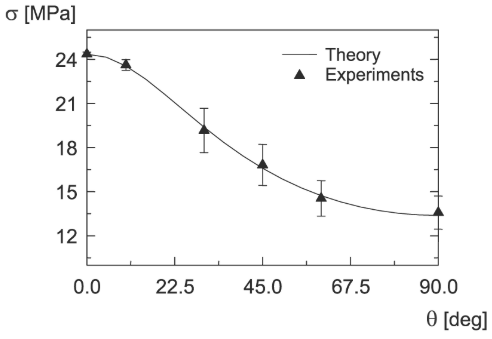
\includegraphics[width=0.5\textwidth]{chapter_2/figures/Orientation.PNG}
    \caption{Orientations of roads with respect to load applied \cite{Rodriguez2003MechanicalModeling}}
    \label{fig:Orientation}
\end{figure}

The part will have the best mechanical behaviour if it is loaded along the axis direction of the deposited roads. Subsequently, stacking the layers in  $[45/-45]_n$ configuration will result in quasi isotropic properties.

Additionally, not only the raster orientation, but the part orientation significantly influence the part properties. The printbed is in general oriented according to Cartesian coordinates, y being the longitudinal horizontal direction , y the transverse horizontal direction, and z the vertical direction (as can be seen in figure \ref{fig:coordinates}. When defining the angle of the roads, the slicers use the y direction as principal direction, meaning a [0] road will be directed along the y axis, while [90] will be directed along the x direction. 

%%% replace with ASTM F2971

\begin{figure}[H]
    \centering
    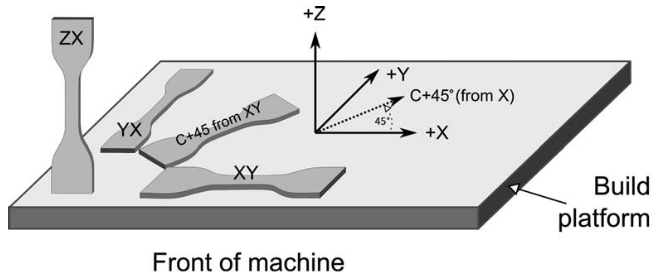
\includegraphics[width=0.4\textwidth]{chapter_2/figures/Coordinates.png}
    \caption{FFF coördinates for test specimen production}
    \label{fig:coordinates}
\end{figure}


\section{Materials}
There is currently a wide range of polymer blends available for FFF, these can also include reinforced particles. The nature of the process, liquefying the polymer, only allows for thermoplastics. Thermosets have cross-links connecting the polymer chains, causing the material to degrade rather than to flow when heated. Parameters and properties such as crystallinity, $T_m$, $T_g$ and the thermal expansion coefficient make certain polymers more applicable for FFF.  A deep comparison of different polymers and their properties will not be part of this thesis. A concise analysis and substantiation for the material that will be used in this thesis will be presented in this chapter.

\subsection{Materials for FFF}
In figure \ref{fig:pyramidpolymer} the different thermoplastic polymers can be seen. The y-axis represents the performance of the material, often related to the cost and ease of use. Be aware that the material properties of bulk or conventional produced polymer differ from the material properties found in the produced part. 

\begin{figure}[H]
    \centering
    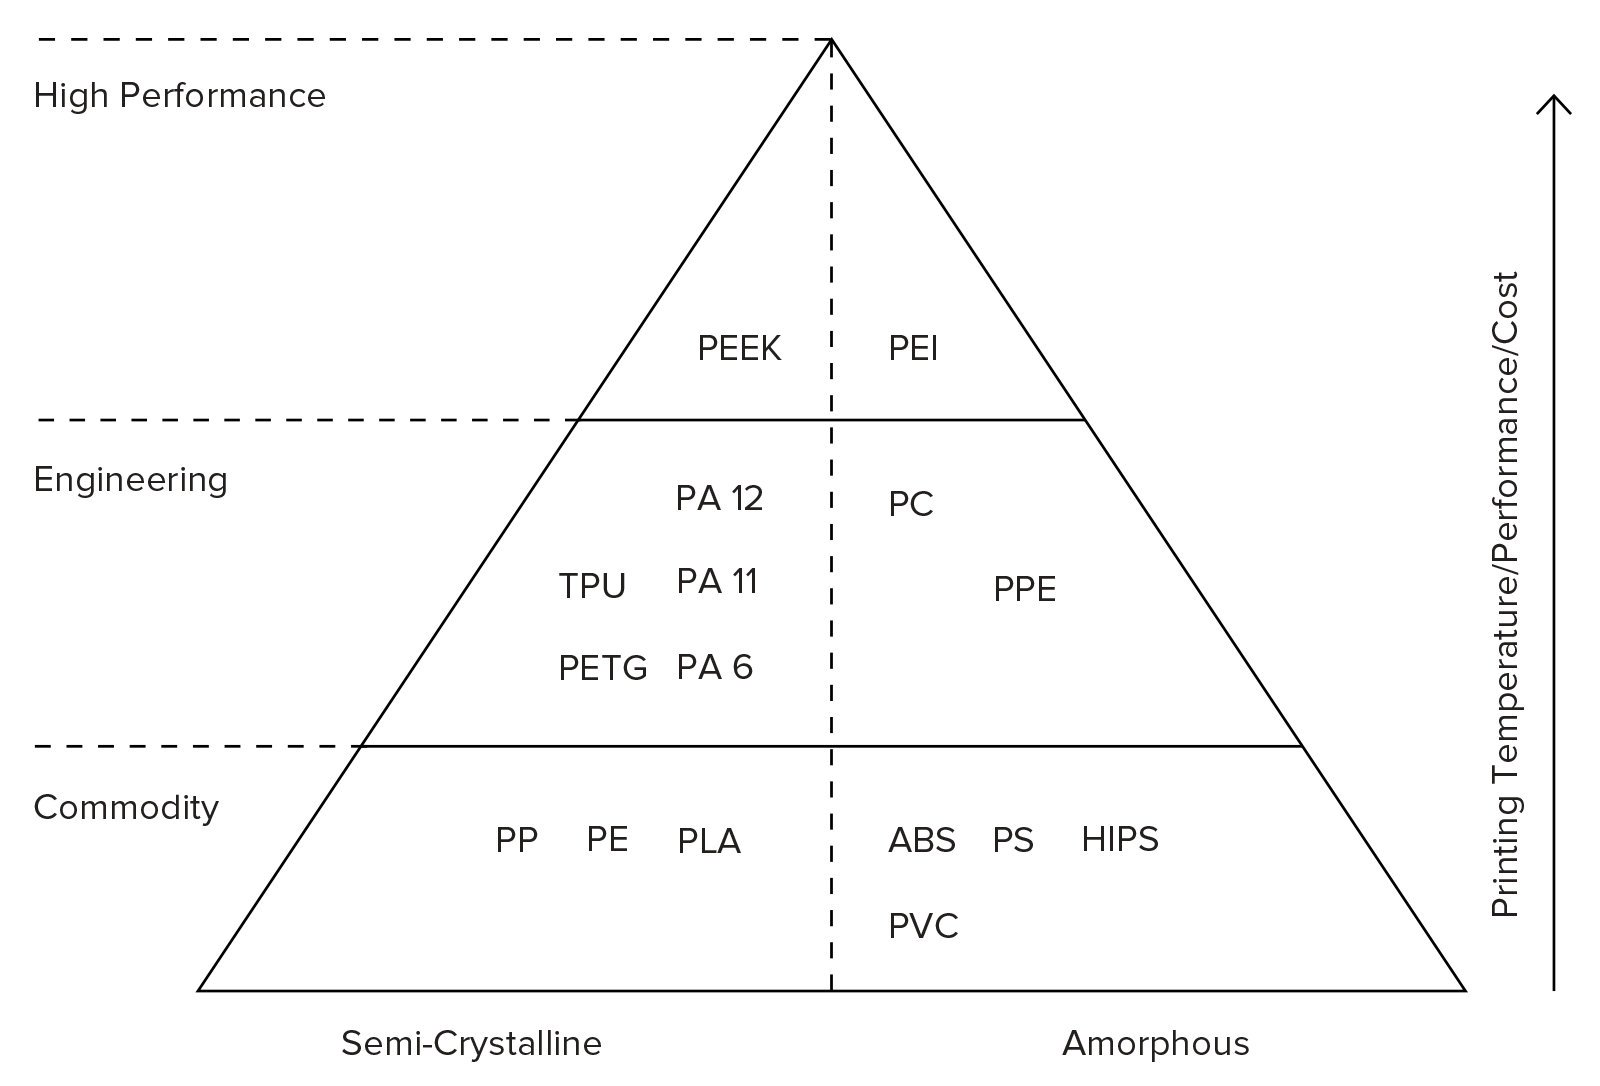
\includegraphics[width=0.6\textwidth]{chapter_2/figures/Pyramidpolymer.png}
    \caption{Polymer pyramid with FFF polymers \cite{Redwood2017TheApplications}}
    \label{fig:pyramidpolymer}
\end{figure}

To create a focus for this thesis, a particular material must be chosen to apply a scope on the research. To identify the mechanical properties of FFF produced parts, and the parameters affecting this, a polymer that has been used and researched extensively should be selected. This leads us to the lower tier of the pyramid, where PLA en ABS are by far the most implemented polymers. This is mostly due to the fact that FFF printers had only the possibility to print PLA and ABS until late 2012 \cite{WohlersAssociates2017WohlersIndustry}, therefore it is not surprising that most systems are optimized for these materials. Since the academic research is limited on the topic of FFF (compared to e.g. injection moulding, which is a technology that has matured for decades), PLA and ABS are the best candidates.

PLA and ABS are most distinguishable by their polymer structure,  PLA is semi-crystalline and ABS is amorphous. This difference is mostly noticable in the thermal/viscous properties \cite{Rodriguez-Panes2018TheAnalysis}. PLA has a clear melting temperature $T_m$ (the moment where the semi-crystalline isotactic chains break its van der Waals forces), while ABS has only a glass transition temperature $T_g$, (where the polymer chains have enough thermal energy to start diffusing and consequently drop its Young's modulus). This phenomenon is pictured in \ref{fig:EvsT}. 

The amount of crystallization can differ through a polymer based on the thermal history. High cooling rates can prevent chains from crystallizing, resulting in a smaller crystalline phase, this is typical for the FFF process. High degree of crystallinity is coupled with harder and thermally stable materials\cite{Balani2015PhysicalPolymers}. The amorphous regions provide elasticity and impact resistance. These properties are also reflected in the properties of PLA and ABS. 

The temperature history is dependant on the process parameters and geometry, resulting in an even larger fluctuation in mechanical properties when comparing different studies. This also means that it will be harder to generate constant samples and products with semi-crystalline polymers. Additionally, Peterson \cite{Peterson2019ReviewPerspective} confirms this with the following statements; "due to the high cooling rates (in the order of 10K/s) polymers experience: 1) trapping polymers in non-equilibrium conformations; 2) limited time for polymer diffusion at road interfaces; 3) complex (in-unifromaly) crystallization profiles for semi-crysalline polymers". Crystallinity of polymers is extensively discussed in the books on polymer science by Vegt \cite{Van_der_Vegt2001FromPlastics} and Halary \cite{Halary2011PolymerMaterials}.

\begin{figure}[H]
    \centering
    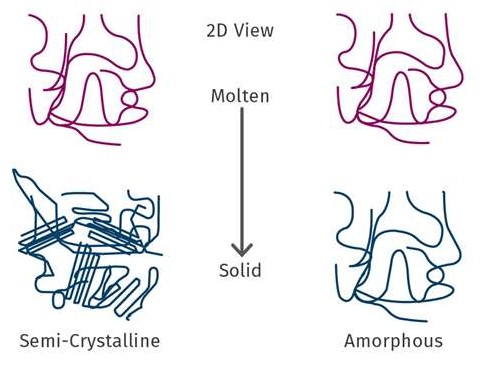
\includegraphics[width=0.4\textwidth]{chapter_2/figures/structurepolymers.PNG}
    \caption{Molecule structure in molten and solid state \cite{PtolinePolymersCrystalline}}
    \label{fig:structurepolymers}
\end{figure}

\begin{figure}[H]
    \centering
    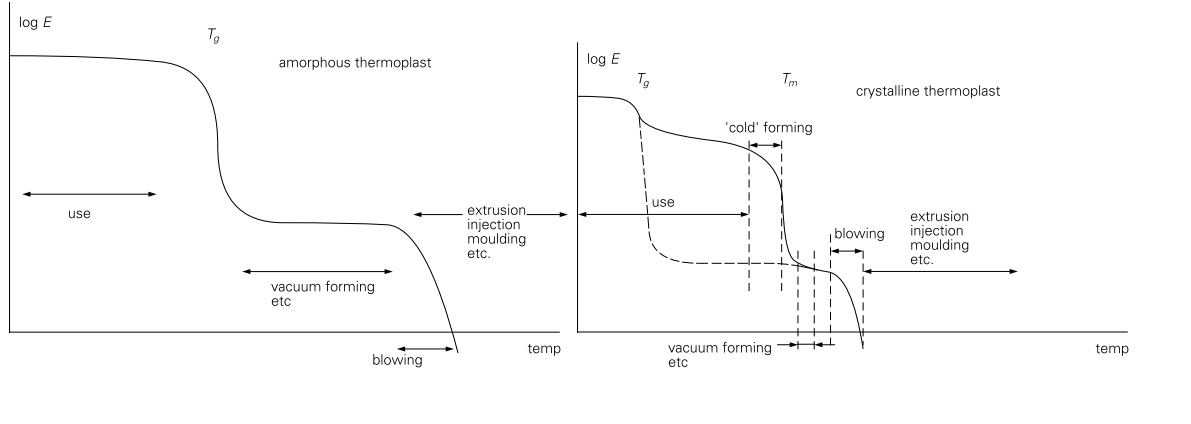
\includegraphics[width=1\textwidth]{chapter_2/figures/EvsT.PNG}
    \caption{E modulus against temperature for amorphous and semi-crystalline polymers \cite{Van_der_Vegt2001FromPlastics}}
    \label{fig:EvsT}
\end{figure}

Despite that PLA is gaining popularity, due to its ease of use, low cost and biodegradability, it has limited scientific backed research compared to ABS. ABS has been used more extensively in different production methods (e.g. injection moulding). Especially with the systems of Stratasys (which were optimized for ABS P400) a lot of research was done. Popescu et al. \cite{Popescu2018FDMReview} reviewed a large amount of articles related to the mechanical properties of FFF printed parts, additionally Mohamed et al. \cite{Mohamed2015OptimizationProspects} and Peterson \cite{Peterson2019ReviewPerspective} did a similar review on the empirical research that has been done, all results are in line with previous statements.  

Taking into account the physical issues with semi-crystalline polymers and the abundance of research presented on ABS, the choice to focus this thesis on ABS is substantiated.

\subsection{ABS properties}
    \label{ABS properties}
 \subsubsection{Chemical composition}
As stated before, ABS (Acrylonitrile Butadiene Styrene $(C_8H_8)x (C_4H_6)y (C_3H_3N)z)$ is a amorphous thermoplastic with a glass transition temperature of approximately 105$^{\circ}$C \cite{Peterson2019ReviewPerspective}. Due to it's amorphous nature it has no true melting point, therefore there is no sudden viscosity drop. It is a terpolymer (build from three monomers), and is created by polymerizing styrene and acrylonitrile in the presence of polybutadiene, figure \ref{fig:ABSforumla}.

\begin{figure}[H]
    \centering
    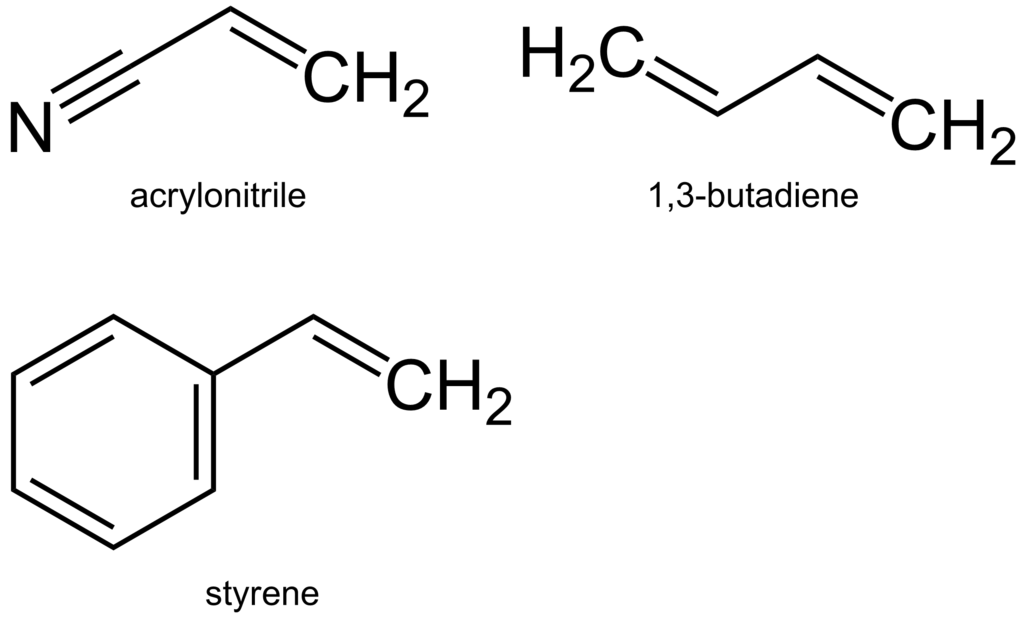
\includegraphics[width=0.4\textwidth]{chapter_2/figures/ABSformula.PNG}
    \caption{Monomers in ABS polymer}
    \label{fig:ABSforumla}
\end{figure}
The proportions of the different monomers vary for Acrylonitrile from 15-35\%, which gives thermal and chemical resistance,  butadiene from 5-30\%, which gives toughness and performance over a broad temperature range and styrene 40-60\%, which is cheap, eases process-ability, machine-ability and produces high gloss \cite{GrantaDesignLimited2018CESEdupack}. This results in a long chain of polybutadiene criss-crossed with shorter chains of poly(styrene-co-acrylonitrile). ABS has a general service temperature between -30 and 70 degrees, which means that the mechanical properties in use should not differ significantly in this range. An extensive study is presented by Peterson on the ABS blends and their properties for FFF \cite{Peterson2019ReviewPerspective}.

\subsubsection{General properties}
ABS is often used due to its low cost, high impact resistance (also at low temperatures) and decent mechanical properties. It is also easy to color, is scratch and scuff resistant, and is easily processed and bonded \cite{GrantaDesignLimited2018CESEdupack}. According to CES edupack \cite{GrantaDesignLimited2018CESEdupack} general purpose extrusion ABS has low shrinkage and warpage. However, for FFF applications, ABS is difficult to use due to it's high warpage (in comparison to PLA). 
ABS has furthermore good resistance against chemicals and  solvents and is a decent electrical insulator. The thermal process parameters (regardless of FFF) have  effect on other properties of the ABS polymer, high temperature processes improve the gloss and heat resistance, while low temperatures increase impact resistance and strength. 
The limiting factors of ABS are its poor resistance to UV light and it's low operating temperature. The concentration of polybutadiene can increases the aging characteristics while other additives increase UV-protection. ABS is also suitable for additives such as glass and carbon fibers. 

\subsubsection{Molecular structure}
	%Reptation (healing etc)
    Thermoplastic amorphous ABS looks on a molecular scale like a spaghetti of unchained polymers, as can be seen in figure  \ref{fig:structurepolymers}. The polymers belonging to this class of materials are characterized by the temperature dependence of the Young modulus shown in figure \ref{fig:EvsT}. Each polymer chain adopts a coil conformation that strongly overlaps with its neighbors leading to chain entanglements. The entanglement density, $\nu_e$, is an important characteristic that affects the toughness of the polymer significantly, and is defined as the number of entanglements per unit volume of the material:

\begin{equation} \label{eqn:Me}
\nu_e=\frac{N_A\rho}{M_e}
\end{equation}

where $\rho$ is the polymer density, $M_e$ the molecular weight of the chain between two entanglements, $N_a$ the Avogadro number\cite{Halary2011PolymerMaterials}. 

Amorphous polymers show a significant drop in stiffness after the glass transition temperature. According to Appelsved \cite{Appelsved2012InvestigationModels}, this is the moment where the inter molecular bonds (van der Waals) break, after this moment the chains are able to diffuse through the polymer blend. 
For samples with a molecular weight higher than the molecular weight between entanglements, $M_e$, the Young modulus decreases through the glass transition and reaches a plateau value of about 1 MPa. This is called the rubberey plateau and its extent increases with molecular weight. At higher temperatures these high molecular weight polymers go trough a fluidification zone before becoming highly viscous liquids. This is consequently the phase of material where the material is extruded. If  $M$ is smaller than $M_e$, the polymer skips the rubbery plateau, and almost immediately forms a viscous liquid. A relation between the temperature molecular weight and phase is shown in figure \ref{fig:polymerphase} \cite{Halary2011PolymerMaterials}.

\begin{figure}[H]
    \centering
    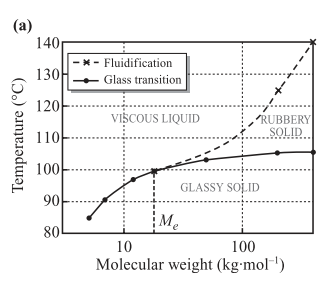
\includegraphics[width=0.4\textwidth]{chapter_2/figures/polymerphases.PNG}
    \caption{State diagram of un-cross-linked amorphous cis-1,4-polyisoprene \cite{Halary2011PolymerMaterials}}
    \label{fig:polymerphase}
\end{figure}
Reptation is possible when $M_e$ is smaller than $M$, and occurs after the glass transition temperature. The simplest form of the model assumes the polymer being "trapped" by entanglements, which is analogous to a chain trapped in a tube. The effective distance to free itself from the original entanglements is equivalent to the chain length. The speed at which the chain can reptate out of its entanglements is related to the temperature of the polymer blend\cite{Halary2011PolymerMaterials}.  
Thermoplastics inhibit inherent viscoelasticity, also called creep, which describes the phenomenon of molecule diffusion under an applied load. This mechanism is quite difficult to predict, and will not have a focus in this thesis. Most important to notice is the significant effect of the strain rate on the mechanical response of thermoplastics, as is shown in figure \ref{fig:Strainrate}.
When extruding or processing thermoplastics, chains are being broken and reduced in length, this decrease in molecular weight leads to alteration of the response under different temperatures as is shown in \ref{fig:polymerphase}.

% Mechanical behaviour
\subsection{Elasticity}
Polymers exhibit an elastic response to a loading that is defined as instantaneous and reversible and may have either an energetic or an entropic physical origin. These constitutive mechanism are designated as true elasticity and hyper elasticity respectively. True elasticity, which for polymers only occurs at low strains, is linked to a poisson ratio that varies between 0.3 at low temperature and 0.5 at temperatures equal to or higher than the glass transition temperature. 
The entropic effect describes the increase in entropic energy (heat) of the polymer chain as a larger force due to the dynamic movement of the molecule. 
Random coils can be considered as a spring, multiple springs are connected to each other through entanglements. Thermosets, which contain crosslinks, have more predictable elastic behaviour than thermoplastics, which inhibit a large amount of viscoelasticity. However, these entanglements have similarities to cross links in the glassy state at a low strain, these enthanglements will dissapear as a result of sliding motion of the chain. Different models exists to predict the elastic behaviour of polymers, especially for thermosets, these are defined in detailed in the book of Halary \cite{Halary2011PolymerMaterials}. If we consider the stress strain curve of a typical thermoplast from figure\ref{fig:SSpolymers}, we observe a quasi-linear region up to the top of the curve where $d\sigma/d\epsilon=0$. This top is defined as the yield point for thermoplastics \cite{NEN-EN-ISO2016NEN-EN-ISO527-2}, which differs from the definition for e.g. metals. According to Appelsved \cite{Appelsved2012InvestigationModels} the true yield point of polymers is the stress at which van der Waals bonds are all broken, and chains can diffuse freely.  

\begin{figure}[H]
    \centering
    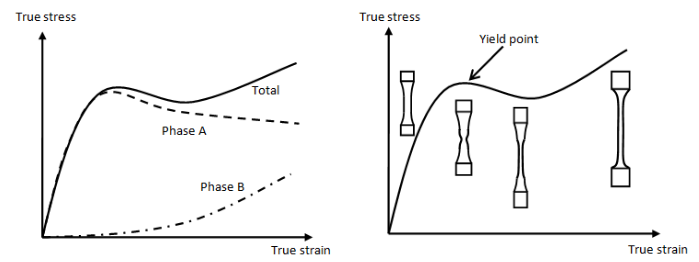
\includegraphics[width=0.6\textwidth]{chapter_2/figures/SSpolymers.PNG}
    \caption{Typical stress-strain curves for thermoplastics \cite{Appelsved2012InvestigationModels}}
    \label{fig:SSpolymers}
\end{figure}
Additionally, Appelsved differentiates two different phases (figure \ref{fig:SSpolymers}); phase A which dominates up to the stress maxima and deformation is mainly generated from movement of the molecular chains relatively to each other. Eventually the bonds break and the slope decreases. Since a polymer blend is a distribution of chains with different lengths, this is expected to occur over a strain range instead of a sudden drop. After the bonds are broken strain softening occurs. In phase B, the molecule chain itself is straightened, resulting in re-hardening at larger strains. The alignment at large strains cause transverse isotropy. The straightening of the molecular chains makes the material stronger, resulting in a different necking behaviour in contrast to metals. 

\begin{figure}[H]
    \centering
    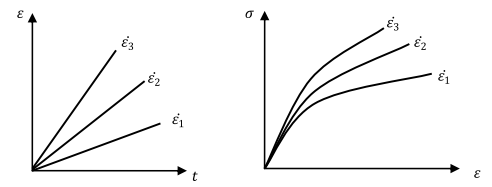
\includegraphics[width=0.5\textwidth]{chapter_2/figures/Strainrate.PNG}
    \caption{Effect of strain rate dependency on polymers \cite{Appelsved2012InvestigationModels}}
    \label{fig:Strainrate}
\end{figure}
\subsection{Plasticity, damage and failure}
Due to the molecular structure of polymers, it is difficult to determine the start of plasticity. Loading/unloading experiments can be carried out to determine irreversible strains.  The effect of loading and un-loading is depicted in figure \ref{fig:Irr}. The unloading is followed by recovery, until the residual strain have stabilized and can be concluded as permanent.
\begin{figure}[H]
    \centering
    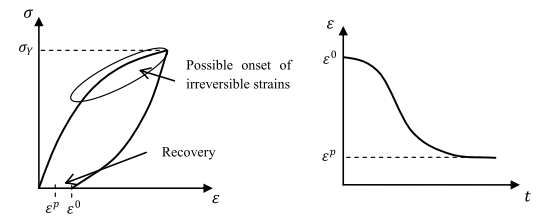
\includegraphics[width=0.5\textwidth]{chapter_2/figures/Irr.PNG}
    \caption{Loading/unloading behaviour with recovery \cite{Appelsved2012InvestigationModels}}
    \label{fig:Irr}
\end{figure}
Halary \cite{Halary2011PolymerMaterials} claims that conducting compressive tests have the advantage of avoiding the effect of micro-voids always present in samples, since these voids increase sample brittleness on tensile straining. 
In figure \ref{fig:SSPMMA} empirically generated uniaxial compression stress strain curve of an amorphous thermoplastic polymer (PMMA) can be seen. The slope of the straight line corresponds to the material Young's modulus. Between A and B the stress-strain relation is no longer linear and the material exhibits an anelastic behaviour. In figure \ref{fig:SSresidual} a schematic drawing of different loading regions is shown to support the explanation. In this region strain is still reversible. 
After the stress maximum at the yield point, a clear viscoplastic behaviour occurs. Additional strain is irreversible, and will lead to residual strain after unloading. It is worth pointing out that these residual strains can be removed by heating the polymer sample above its glass transition temperature. In general, it can be assumed that the Young's modulus remains relatively similar up to the plastic range. 

\begin{figure}[H]
    \centering
    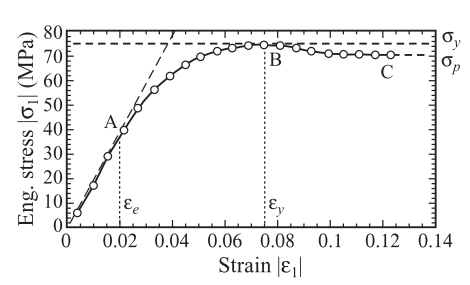
\includegraphics[width=0.5\textwidth]{chapter_2/figures/SSPMMA.png}
    \caption{Compression stress-strain curve of a PMMA (A, elastic limit; B,yield point; C, plastic flow)\cite{Halary2011PolymerMaterials}}
    \label{fig:SSPMMA}
   \end{figure}
\begin{figure}[H]
    \centering
    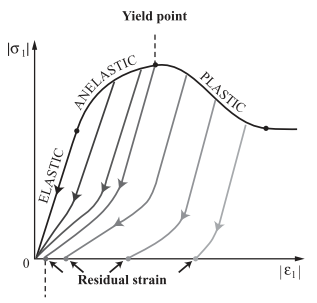
\includegraphics[width=0.4\textwidth]{chapter_2/figures/SSresidual.png}
    \caption{Schematic drawings of unloading profiles for a sample compressed at various strain values.)\cite{Halary2011PolymerMaterials}}
    \label{fig:SSresidual}
   \end{figure}
%\subsubsection{Yielding}
\subsubsection{Yielding}
%\subsubsection{Dependency on Hydrostatic stress (models)}
Most common yield and failure criteria, like von Mises and Tresca \cite{Christensen2013TheFailure}, are dependent on the stress state of the material. This stress state is a function of the von Mises ($\sigma_v$) or equivalent stress:

\begin{equation}\label{von mises}
\sigma_v=\sqrt{\frac{(\sigma_{11}-\sigma_{22})^2+(\sigma_{22}-\sigma_{33})^2+(\sigma_{33}-\sigma_{11})^2 +6(\sigma_{23}^2+\sigma_{13}^2+\sigma_{12}^2)}{2}} 
\end{equation}


However, these do not include dependency on the hydro-static stress, which is most common for metals. Yield and failure criterion for polymers are generally dependent on the the hydrostatic stress ($\sigma_h$):
\begin{equation} \label{eqn:Me}
  \sigma_h=P=\frac{\sigma_x+\sigma_y+\sigma_z}{3}
\end{equation}
Additionally the yield and failure are criterion are a function of the the stress triaxiality ($\sigma_t$):
\begin{equation}\label{AzziTsai}
\sigma_t=\frac{\sigma_h}{\sigma_v}
\end{equation}
The difference in yield and failure loci can be observed in figure \ref{fig:yieldloci}.
\begin{figure}[H]
    \centering
    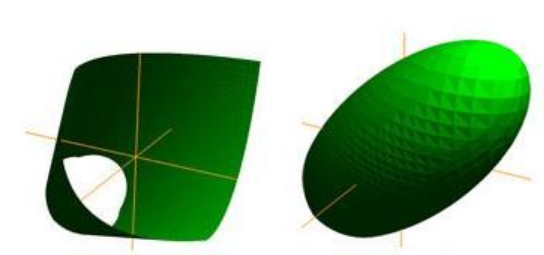
\includegraphics[width=0.5\textwidth]{chapter_2/figures/yieldloci.png}
    \caption{Failure locus for metals (left), and for ductile polymers (right), with the axis corresponding to the principal directions \cite{Christensen2013TheFailure}}
    \label{fig:yieldloci}
\end{figure}
The axis in this figure represent the principal stress directions. The left surface is defined by a stress state of the von Mises stress. If a pure hydrostatic pressure is applied, the surface will not be crossed. For polymers there is also a dependency on the hydro static pressure, since it will cross the surface at some point.  
It should me mentioned that the yield and failure surface for polymers is in reality not symmetric for tension and compression, as can be seen in figure \ref{fig:SStensioncompression}. It has been concluded by several books on failure mechanics \cite{Michael1985FractureMechanics}\cite{Christensen2013TheFailure} that polymers have a higher compressive yield strength than in tension. 
For ductile polymers also failure criteria are used based on the equivalent strain. This strain is calculated in a similar way as the equivalent stress. The failure surface might differ from the conventional von Mises or Tresca surfaces. 
\begin{figure}[H]
    \centering
    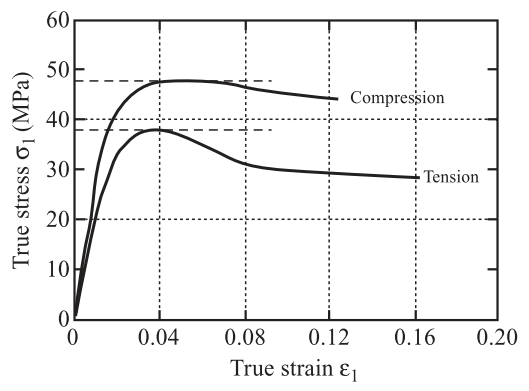
\includegraphics[width=0.4\textwidth]{chapter_2/figures/SStensioncompression.png}
    \caption{Comparison of stress-strain curves for PMMA for compression and tension \cite{Halary2011PolymerMaterials}}
    \label{fig:SStensioncompression}
\end{figure}

Assuming a isotropic polymer blend of ABS, we need to define a yield function based on the principal stress state of the material, $f(\sigma_1,\sigma_2,\sigma_3)$ that is also dependant on the on the hydrostatic pressure. 
Claiming that a material has hydrostatic pressure sensitivity permits us to write the stress tensor as the sum of its deviatoric $\sigma_p$, and volumetric stress (the identity matrix multiplied with the hydrostatic stress) components, as expressed in equation \ref{eqn:deviatoric}:
\begin{equation}\label{eqn:deviatoric}
\begin{vmatrix}
\sigma_{1}&0&0\\
0&\sigma_{2}&0\\
0&0&\sigma_{3}\\
\end{vmatrix}
=
\begin{vmatrix}
\sigma_{1}-P&0&0\\
0&\sigma_{2}-P&0\\
0&0&\sigma_{3}-P\\
\end{vmatrix}
+
\begin{vmatrix}
P&0&0\\
0&P&0\\
0&0&P\\
\end{vmatrix}
= \sigma_d+\sigma_h\cdotI
\end{equation}Where $I$ is the identity matrix.  
An enhanced form of the von Mises criterion can then be applied to polymers in the following way:
\begin{equation} \label{eqn:yieldpolymers}
  (\sigma_{11}-\sigma_{22})^2+(\sigma_{22}-\sigma_{33})^2+(\sigma_{33}-\sigma_{11})^2=(2\sigma_y+\mu_{vM} \cdot \sigma_h)^2
\end{equation}
Where $\mu_{vM}$ is an internal friction coefficient. The corresponding plasticity envelope is a cone whose axis is the hydrostatic pressure axis, and whose axis increases with hyrdrostatic pressure, similar to the yield locus for polymers in figure \ref{fig:yieldloci}. A similar procedure can be applied to the tresca criterion. 

\begin{figure}[H]
    \centering
    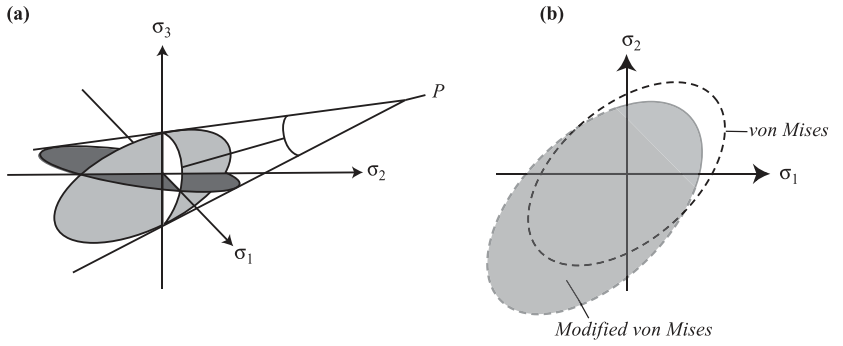
\includegraphics[width=0.75\textwidth]{chapter_2/figures/yieldpolymers.png}
    \caption{Yield surface for polymers a) three-dimensional b) two-dimensional compared with von Mises \cite{Halary2011PolymerMaterials} }
    \label{fig:Midplane}
\end{figure}

%Ree-Eyring
The Ree-Eyring model explains the yield behaviour on a molecular scale, according to this model, the sliding of molecules with respect to each other is achieved by passing through a transition state, called activated state, overcoming an energy barrier depending on both temperature and applied stress. This models assumes plastic deformation of amorphous polymers is occurs as the displacement of chain segments from a site A to a site B due to an activation state, related to energy $\Delta G$, both located in a sliding plane resulting from the presence of a shear component. The principle of the model can be seen in figure \ref{fig:Ree-Eyring}. In the anelastic range the chains are merely "stretched" and will not permanently displaced with respect to the other chains in the blend. In comparison with the theory presented by Apselveld, one could argue that the "activation energy" for permanent displacement is analogous to the breaking of the van der Waals bonds.

\begin{figure}[H]
    \centering
    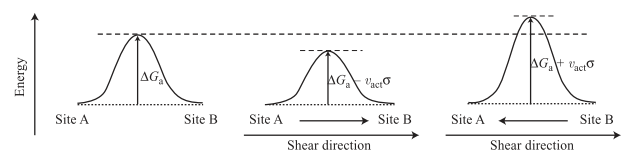
\includegraphics[width=0.8\textwidth]{chapter_2/figures/Ree-Eyring.png}
    \caption{Energy diagram showing the principle of the Ree-Eyring model \cite{Halary2011PolymerMaterials}}
    \label{fig:Ree-Eyring}
\end{figure}
%plastic instability
During tensile tests beyond the yield point many polymers, including amorphous polymers, undergo a plastic instability, the necking phenomenon. In this plastic region, chains have reached their extensibility limit, further neck propagation occurs trough neighboring regions. After development of the whole neck propagation a uniform strain occurs again, until the sample breaks as can be seen in figure \ref{fig:Necking}. In figure stable necking is observed, while in figure b unstable necking leads to quick fracture. This behaviour depends on the considered polymer, possible defects, temperature and strain rate conditions. 
\begin{figure}[H]
    \centering
    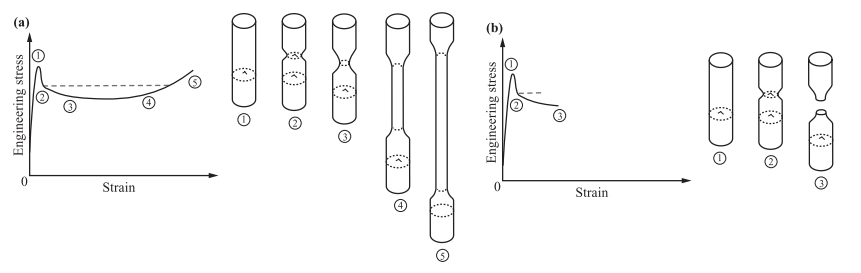
\includegraphics[width=1\textwidth]{chapter_2/figures/Necking.jpg}
    \caption{Schematic drawing of the necking phenomenon \cite{Halary2011PolymerMaterials}}
    \label{fig:Necking}
\end{figure}
There exists several yield and failure criteria for thermosets and composites. Since thermoplastics have a more complex behaviour due to their viscoeleasticity in this section the different models will be discussed. 
Lin\cite{Lin2013StressLoading} confirms the lack of accurate yielding and failure criteria for thermoplastics. Additionally, the PhD. thesis of Melick \cite{Melick2002DeformationGlasses} on the deformation and fracture of polymer glasses also mention the lack of failure criterion, and does not produce a satisfying solution for this issue. Different  models (brittle or ductile) are implemented in commercial software such a as the equivalent strain criterion, von Mises, Johnson-Cook, Hill and Drucker-Prager. The main drawback in these fracture models is that accurate predictions of failure can only be achieved for limited stress state and strain rate, which cannot be applied for thermoplastics. One of the currently popular material models for polymer plasticity  in LS-DYNA is SAMP-1 (semi analytical model for polymers)

Melro \cite{Melro2013MicromechanicalModelling} proposes a paraboloidal yield criterion for epoxies defined by Tschoegl, which can be defined as:
\begin{equation}\label{eqn:Tschoegl}
\Phi=6J_2+2I_1(\sigma_c-\sigma_t)-2\sigma_c\sigma_t
\end{equation}Where $J_2$ is the second invariant of the deviatoric stress tensor, and $I_1 = tr(\textbf{\sigma})$. This is a variation of the general yield criterion shown in equation \ref{eqn:yieldpolymers}

Du Bois \cite{DuBois2006APolymers} implemented a seminanalytical model \ref{eqn:DuBois} for the simulation of polymers (SAMP-1) in LS-DYNA under MAT187. 
\begin{equation}\label{eqn:DuBois}
f=\sigma_v^2-A_0-A_1\cdot \sigma_h-A_2\cdot p^2<0
\end{equation}For further details the reader is referred to the mentioned article. 

Another popular yield criterion that is used by the SAMP-1 material model in LS-DYNA is that Drucker-Prager yield criterion. 

\subsubsection{Damage and failure}
Damage and fracture are important to investigate to identify the failure mechanism of the polymer, both concepts cannot be dealt with separately, since fracture, which results in the sample breakdown, usually comes after damage. Depending on the deformation conditions (stress field, temperature, strain rate) and characteristics of the polymer chains (chemical structure, molecular weight), two types of deformations may occur: shear bands and crazes. Shear bands are deformations in shear direction (45 degrees for uniaxial compression tension), important to note is that they do not create any voids inside the material, and therefore will not induce and volume change. Shear band growth is controlled by plastic sliding only, therefore, stress associated with shear band formation is assumed to be equal to the yield stress. 

%crazes
Crazes are small microvoids containing fibrils bridging the two craze faces. Such fibrils play a major role in the ability of the craze to sustain loading in the direction perpendicular to its faces. These microvoids are ellipsoidal heterogeneities with a size ranging from 10 $\mu$m to 10 mm along the major axis and from 1 to 10 $\mu$m in along the minor axis. In figure \ref{fig:Craze} a schematically image is shown of crazes. The ratio between crazes an fibrils are approximately equal.  

\begin{figure}[H]
    \centering
    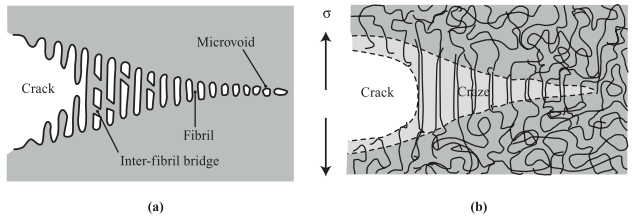
\includegraphics[width=0.8\textwidth]{chapter_2/figures/Craze.png}
    \caption{Schematic drawing of a craze a) Microvoids b) conformations of chains within a craze \cite{Halary2011PolymerMaterials}}
    \label{fig:Craze}
\end{figure}
A crack systematically initiates from a sample "defect". Despite a crack being inherently different from a craze, a craze initiates from microvoids. These defect lead to stress concentrations allowing the craze to grow, but only at temperatures under the glass transition temperature. These stress concentrations can be predicted by conventional fracture mechanics, this will be further investigated in chapter 7. Fibrils in the crazes may either break, which requires to break high energy covalent bonds, or when undergoing higher mobility, may slide with respect to each other. The first results when high strain rate is applied at low temperature, and the latter occurs at a temperature near $T_g$. These mechanisms occur under tension at a stress lower than yield stress, and grow perpendicularly to the direction of the highest principal stress.
A craze criterion is proposed based on two arguments:
- Crazes are formed when strain reaches a critical value, $\epsilon_c$, along one principal direction.
- This strain craze value, which varies with temperature and strain rate, depends on the hydrostatic component of the stress tensor according to:
\begin{equation} \label{eqn:crazecriterion}
 \epsilon_c=Y+\frac{X}{\sigma_1+\sigma_2+\sigma_3}
\end{equation}
%adding strain surface??
Where X an Y are experimental parameters. From this criterion an envelope can be made to compare it with the von Mises yield criterion as can be seen in figure \ref{fig:crazecrit}. 

\begin{figure}[H]
    \centering
    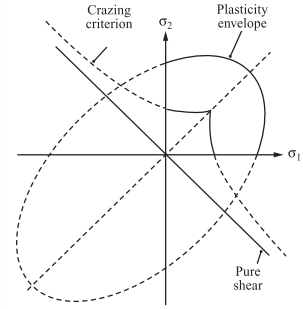
\includegraphics[width=0.3\textwidth]{chapter_2/figures/crazecrit.png}
    \caption{Plasticity envelope and craze criterion for PMMA \cite{Halary2011PolymerMaterials}}
    \label{fig:crazecrit}
\end{figure}

The craze strain criterion can occur before yielding and plasticity, whereas shear bands only occur beyond the plasticity threshold. This result implies that any combination of two tensile stresses generates crazes instead of shear bands. A combination of a tensile and compressive stress might lead to both, pure compression always generates shear bands.
To discriminate between shear bands and crazes, one could perform optical microscopy. Extensive research was conducted on this topic, the general conclusions are that the type of damage (crazing or shear bands) are dependant on the polymer, stress state, and temperature. In amorphous thermoplastics, both can be identified by the whitish color due to the scattering of light trough polymer alignment. This effect is more intense for crazing, as a result of the higher density, and is more localized for shear banding.
Additionally interactions may exist between these two types of damage. Initiation of shear deformation zones at the craze tip can occur when the craze propagation rate and widening are small. 

Halary et al. concluded that despite the issues with microvoids, the uniaxial tensile test and uniaxial compressive tensile test have a generally identical shape and domains. Fracture occurs in the viscoplastic domain, it is a ductile fracture with a specific angle of about 45 degrees between the fracture line and stretching direction. At lower temperatures, fracture generally takes place in the anelastic domain, there might be overlap with theory concerning brittle fracture of metals at low temperatures.  

In FEM modelling software different damage and failure models are implemented. The damage initiation point defines start of degradation of stiffness, it only leads to effective damage if damage evolution is specified \cite{ABAQUS2006MaterialFailure}. In case of ductile damage, D is a function of plastic straining and affect the yield stress rather than the elastic modulus. This is equivalent to plastic softening. The material point is assumed to fail when the overall damage variable D reaches a critical value $D_{max}$.
A general form of the strain based fracture loci for thermoplastics can be written as follows
\begin{equation}\label{AzziTsai}
\bar{\epsilon_f}=f(\eta)=f\left(\frac{\sigma_h}{\sigma_v}\right)
\end{equation}
%In the SAMP-1 a simple damage model was added where the damage parameter D is a function of plastic strain only. In this model a load cuve must be provided by the user giving D as a function of the plastic strain under uniaxial tension. The value of the critical damage $D_c$ leading to rupture is then the only other required additional input, this model behaves istropically. Furthermore the model uses the notion of the effective cross section, which is the true cross section of the material minus the cracks that have happened. 
%This models assumes the start of damage from the yield point, and fails when the damage parameter D drops to 0.   

where $\bar\epsilon_f$ is the equivalent strain at failure. 
%maybe implement equivalent strain here
One of the most popular fracture and damage models for polymers is the Johnson Cook model, widely implemented in ABAQUS and LS-DYNA softaware:

\begin{equation}\label{AzziTsai}
\bar\epsilon_f=\left(D_1+D_2\cdot \exp{\left(D_3\cdot\frac{\sigma_h}{\sigma_v}\right)}\right)\cdot\left(1+D_4\cdot\frac{\dot{\epsilon}}{\dot{\epsilon}}\right)
\end{equation}
where $D_i$ are material parameters\cite{DuBois2006APolymers}, the Hancock-McKenzie approach defines the following parameters: $D_1=0, D_2=3/2, D_3=\epsilon_{1f}\cdotexp(-1/2)$. Additionally, a paper by Gao \cite{Gao2013CriticalPipelines} proposes a different variant of the Johnson Cook criterion:

\begin{equation}\label{eqn:JC}
\bar\epsilon_{f}=1.65\cdot\epsilon_{1f}{\left(-\frac{3}{2}\cdot\frac{\sigma_h}{\sigma_v}\right)}
\end{equation}Where $\epsilon_{1f}$ is the critical strain for ductile materials at which crack are initiated under tension in one direction. Different strain based failure criteria are proposed in LS-DYNA and abaqus. Most implement a simple plastic strain at failure ($\epsilon_p<\epsilon_{pf}$) or a major strain failure ($\epsilon_1<\epsilon_{1f}$), and others use the Johnson-Cook criterion as is described.  

Damage in combination with the Johnson Cook model is defined in material model SAMP-1 in LS-DYNA as:

\begin{equation}\label{AzziTsai}
D=\epsilon_p/\epsilon_f\Rightarrow D<D_c\Rightarrow\epsilon_p<\epsilon_{pf}=D_c\cdot\epsilon_f
\end{equation}The influence of stress triaxiality in a strain based failure criterion is important because different states of stress would result in a different equivalent strain at failure\cite{BoisA:}. 
%damage in polymers
A damage variable, denoted as D, quantifies the part of the material cross section that no longer transmits forces (cracks or voids). In the following section, only isotropic damage is considered. Elastic damage affects material stiffness, ductile damage affects material strenght or both material strength and stiffness. This depends on the chosen formulation where two different approaches may be postulated: strain equivalence or energy equivalence. We will be discussing strain equivalence in this section. 

Damage in polymers is relatively hard to model, since different mechanisms play a large role in the determination of damage. A study on the damage behaviour of polymers \cite{Gu2013ExperimentalThermoplastics}, Gu et al. presents different damage functions based on literature and proposes damage functions based on experimental data. 
The general stiffness damage as function of plastic strain is defined as

\begin{equation}\label{stiffnessdamage}
E_{eff}=E_0\cdot(1-D)
\end{equation}Where Nutini and Vitali proposed a simple definition of the damage parameter calculated from the volume strain, since an important characteristic of thermoplastics is the generation of damage (voids and crazes) during plastic volumetric deformation $\epsilon_v$, which is defined as the sum of the principal strains.

\begin{equation}\label{AzziTsai}
D=1-\exp{(-\epsilon_v)}
\end{equation}

In figure \ref{fig:damagepolymer} the results from a loading/unloading experiment was carried out on a polypropylene sample to get more insight on the damage behaviour. 

\begin{figure}[H]
    \centering
    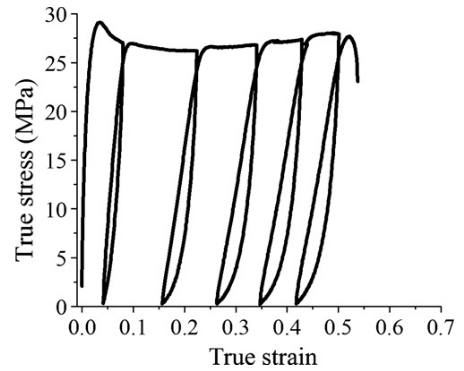
\includegraphics[width=0.4\textwidth]{chapter_2/figures/damagepolymer.png}
    \caption{Sample of trues stress-strain curve of polypropylene\cite{Gu2013ExperimentalThermoplastics} }
    \label{fig:damagepolymer}
\end{figure}
As can be seen, the Young's modulus slightly decreases with plastic strain. However, after the first cycle (just after the softening region) the change in stiffness seems minimal.  Unfortunately, no absolute values of the Young's moduli are presented in this study. 
Following the results, this study proposed a damage function that follows the equation \ref{eqn:stiffnessdamage} fitting the experimental results. Since the damage only occurs in the plastic region for polymers, the result is a function of plastic strain ($\epsilon_p$), and is fitted with a double term exponential function:

\begin{equation}\label{AzziTsai}
D=A\cdot(\exp{(B\cdot\epsilon_p)}-\exp{(D\cdot\epsilon_p))}
\end{equation}The study concludes that the damage parameter calculated with the volumetric deformation underpredicts the damage occurring. A possible reason is that besides voids and crack that might be captured with the volumetric strain, microcracks that do not lead to macroscopic volume change also contribute to damage. 

Christensen \cite{Christensen2013TheFailure}  published a detailed book on failure criteria, but did not take into account materials that exhibit strain softening, therefore his extensive work can unfortunately not be used. 

Rodriguez \cite{Rodriguez2003MechanicalModeling} investigated yield modelling for composite materials under multi-axial loading. He implemented a theory proposed by Tsai-Hill for composites, which is an extension of the von-Mises yield criterion, which defines failure for composites. Originally the Hill theory was developed for anisotropic ductile and brittle materials. Different variations are used for either failure or yield criteria. The  surface is assumed to be quadratic in the stress components. Details on these yield criteria can be found in books on composite mechanical behaviour \cite{Daniel2006EngineeringMaterials}, \cite{Mallick2007Fiber-Composites}.

\subsubsection{Fracture}
Another failure approach is the study of fracture in cracked surfaces. Among the three opening modes, I requires the smallest stress to propagate the notch, therefore, it is considered as the most destructive mode and is often used to estimate the material toughness. A sample weakened by a notch and or crazes will exhibit a lower Young's modulus, therefore, the stress at break, $\sigma_b$ is lowered. On the opposite $\sigma_y$ is only slightly modified. Classical fracture theories can be implemented for crack growth and fracture, these assume a thick plate with a crack of length $2a$. An approach that combines Irwin Criterion and  the approach of Griffith is that a sharp crack can propagate within an finite sample under a critical stress:

\begin{equation} \label{eqn:criticalstress}
 \sigma_{cc}=\frac{K_{Ic}}{\sqrt{(\pi\cdota)}}
\end{equation}
Where $K_{Ic}$ is the critical stress intensity for mode 1 loading. This relates the value of the local stress intensity in the surroundings of the crack tip to the applied loading and is dependant on the material and geometry of the crack. 

The  $K_{Ic}$ has a correlation with the material energy release rate, $G_{Ic}$ under plane strain state, involving the Young modulus and the poisson ratio according to: 

\begin{equation} \label{eqn:crazecriterion}
K_{Ic}=\frac{E\cdotG_{Ic}}{\sqrt{1-v^2_p}}
\end{equation}
Irwin was the first to take into account that stress concentrations at the crack tip may be large enough to move from a local elastic to a plastic response. 

\begin{figure}[H]
    \centering
    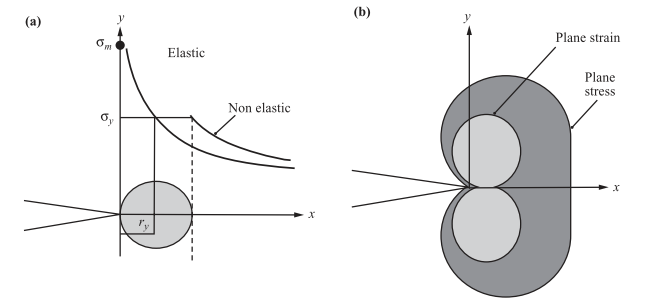
\includegraphics[width=0.8\textwidth]{chapter_2/figures/Crackstress.png}
    \caption{Geometry of the plastic zone a crack tip a) Irwin model b) analysis using von Mises stress\cite{Halary2011PolymerMaterials}}
    \label{fig:stresscrack}
\end{figure}
The radius of the plastic region, $r_y$, as is shown in figure \ref{fig:stresscrack} has been modeled by Irwin under plane strain with the following dependency:

\begin{equation} \label{eqn:cracktip}
r_y=\frac{1}{6\pi}\cdot\left(\frac{K_I}{\sigma_y}\right)^2
\end{equation}There are different ways to calculate $K_{Ic}$ and  $G_{Ic}$, this thesis will not go into detail to determining these values. These values are dependant on numerous polymer characteristics, such as chemical structure, molecular weight, glass transition temperature, etc. It should be noted that the values shift with the thickness of the specimen and is significantly higher for plane stress than for plane strain. Therefore, this method is less appropriate for parts not consisting of plates. 
%Molecular approach of fracture behviour.
Chain entanglements play a fundamental role in fracture properties. Correlations between the fracture properties of polymers and their entanglement density, $v_e$ where found by Halary et al., as can be seen in figure \ref{ref:KIc}.  

\begin{figure}[H]
    \centering
    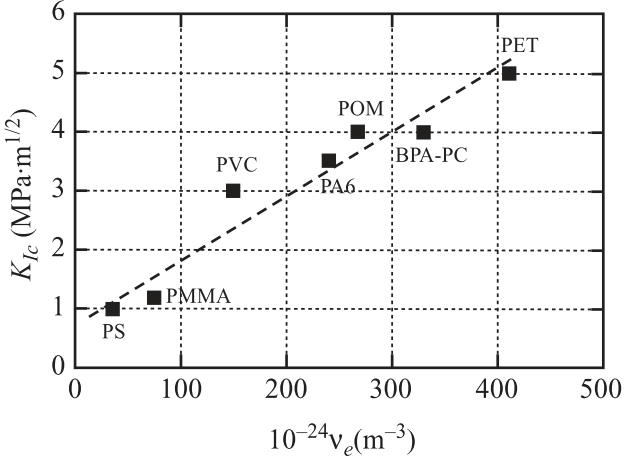
\includegraphics[width=0.4\textwidth]{chapter_2/figures/KIc.png}
    \caption{Correlation between toughness, $K_{Ic}$, and entanglement density, $v_e$  \cite{Halary2011PolymerMaterials}}
    \label{fig:stresscrack}
\end{figure}
These empirical results shows that there is a linear dependence  between the two factors as would be predicted by theory. 

Unfortunately, the work of Halary et al. does not include investigations on ABS polymers. 
%Hergenhahn \cite{Hergenhahn2002FractureABS} has investigated the fracture toughness of ABS for different thicknesses. Following the Izod procedure, the fracture toughness of ABS was found to be 2.8 $MPa\cdotm^{-3/2}$ and for a thickness of 15 mm 2.77. 
Oskui \cite{Oskui2014ExperimentalDevice} determined a fracture toughness of 4.32 $MPa \cdot m^{-3/2}$ for a 10 mm thick specimen. %others also had 4. 

%these analytical models might be appropriate for our problem, but the goal of this thesis is to implement and validate a numerical model, therefore they will not be researched further. 

\subsection{Application of ABS for FFF}
\label{Application of ABS for FFF}
Due to its low glass transition temperature, it's ease of processability, low cost and decent mechanical properties, ABS is a popular polymer to be used for FFF printing of functional parts. Since PLA is even cheaper and easier to use, this polymer is generally used for prototyping and aesthetical parts. Polymers such as PETG, PC and PA are generally used for functional parts. When printing without a heated chamber, polymers with high $T_g$ (for PC 147$^\circ C$) will loose a significant part of their properties due to bad bonding. ABS has a relatively high glass transition temperature ($T_g$ 105), PETG ($T_g$ 80$^\circ C$) and PA ($T_g$ 60$^\circ C$) will have less issues with this. What causes difficulty for the use of ABS with FFF is warping. Coating the build surface with an adhesive will significantly reduce warping.


%the curling of the part (which especially happens for large areas touching the buildplate). This is due to the shrinkage of the first layers that are attached to the bottom layer, this causes the bottom layer to be pulled from the buildplate. To ensure that the part adheres well to buildplate it is essential to have a calibrated "leveled" bed (which determines the distance between the extruder and the buildplate). Also a heated build plate can be incorporated, which drastically limits the thermal gradient between the first layers, reducing thermal stresses. Over cooling the parts with the fans or convection will make your part more prone to warping. A brim (a small entourage of extra roads around the part) is also helpful to stop the part from warping. 
%The extent of warpage is mostly related to the thermal expansion coefficient, $\alpha$, which is around 120 $\mu m/(m C^{\circ}$) according to CES edupack. Even though warpage is an essential part of producing functionally viable parts, it will not be part of this thesis. In future work in this thesis, warpage will not be taken into account. 
It is important to note that the parts produced with FFF are weakest at the inter-laminar interface, and that in different loading conditions the parts most certainly will fail at the laminar interface \cite{Hart2018IncreasedAnnealing} \cite{Popescu2018FDMReview}

\subsection{Standard parameters for ABS}
    \label{standard parameters for ABS}
The technical data sheet of ABS produced by Ultimaker \cite{Ultimaker2018TechnicalABS} assumes the "fine" settings in Cura. These include a 0.4mm nozzle printed at 240-250 C and has a build plate temperature of 85 C, additionally it has a printing speed of 55 mm/s. These settings are recommended for an optimal print, the amount of infill orientation and shell architecture is up to the judgment of the producer. Automatically the slicer produces a shell of about 3 roads thick and applies an infill of 20-50\% filled with a triangle structure. Due to differences in parameters, difference in material and system, lack of standardization, qualification and characterization of results, the produced parts by different researchers will differ widely. Therefor it is difficult to compare the different empirical results from different researchers and datasheets. E.g., the UM datatsheet only states that the printed test specimen are printed in 90\% infill, but the orientation, geometry of the infill and additional parameters have a crucial influence on the mechanical properties of the part. 

\subsection{Standardization}
    \label{Standarization}
In the prior sections it has been made clear that there are a wide range of parameters that can be adjusted. However, there is limited guidance in the standardization of the production process to produce a procedure that can be reproduced. Different researchers have tried to create standardization for their work, generating a multitude of different parameters that are being used, this is well portrayed by review studies such as \cite{Peterson2019ReviewPerspective} and \cite{Popescu2018FDMReview}.  Most plastic producers give relatively little to no information on the process parameters used to test their filament, as can be observed in the Ultimaker ABS datasheet \cite{Ultimaker2018TechnicalABS}. One of the most important characteristics that fluctuate in parts being produced (even if the same process parameters are used), is the healing, wetting and porosity in parts. Although the wetting and porosity can be analyzed by observing the mesostructure, it is extremely hard to characterize the extent of polymer entanglement that will result in road bonding. Employing good hardware (such as a constant envelope heater), reliable sensors and thermocouples and high quality robotics and stepper-motors will generate more consistent results. After a part is produced it can be checked trough some relatively easy steps to determine the quality as described by Tanikella et al. \cite{Tanikella2017TensilePrinting}, e.g. one can weight the produced part to create an estimation for the porosity, and to determine the fluctuation in extrusion by comparing it with the calculated weight by the slicer. Additionally, one could perform a density test by applying the Archimedes principle.

In the past years efforts have been made to use standard printing processes and test procedures. Nist \cite{Forster2015NISTApplicability} published a standard for testing additively manufactured polymer materials, including FFF thermoplastic testing. These test methods advise using either ISO 527-2 \cite{NEN-EN-ISO2016NEN-EN-ISO527-2} or ASTM D638 \cite{ASTM2015ASTMD638-14} for tensile test, which both describe the tensile test for a thermoplastic polymers. They are similar on most points, indicating a geometry and test conditions for the experiments, including a sample size of 5 specimen per test. In general this seems like a decent test method, however, in some cases (due to the large in-isotropic behaviour and nonuniform bonding between roads) the test specimen fails in unexpected ways, often failing at the clamps or the fillets due to stress concentrations\cite{Alaimo2017InfluenceParts}, or having consecutive roads failing due to bad layer bonding and surface roughness \cite{Ahn2002AnisotropicABS} \cite{Bertoldi1998MechanicalDeposition}. 

As an alternative to the ISO 527 or ASTM D638 standard, a composite alternative is proposed by Rodriguez \cite{Rodriguez2001MechanicalInvestigation}, which applies the ASTM D3039 on his tests, which are normally used for long fiber samples. The advantage of this standard is the fact that it does not have fillets at the end of the sample, reducing the stress concentration and possibility for defects.

The document presented by NIST \cite{Forster2015NISTApplicability} still lacks standards on the production of test specimen. Additionally, ISO and ASTM published useful documents on general principles and terminology including ISO 17296  \cite{NEN-EN-ISO2019NEN-EN-ISOTestmethoden} ISO/ASTM 52900 \cite{ASTMInternational2017ISOParts} ISO/ASTM 52901 \cite{2019NEN-EN-ISOParts} ISO/ASTM 52910  \cite{ASTMInternational2017ISOParts} ISO /ASTM 52921 \cite{2019NEN-EN-ISOParts} ASTM F2971 \cite{2013ASTMManufacturing}, the last standard assumes a coordinate system (figure \ref{fig:coordinates}) which will be used for further reference. A book on standards and quality control was presented by Chua et al. \cite{ChuaStandardManufacturing}

Rodriguez \cite{Rodriguez2003MechanicalModeling} has assumed three normal material directions in line with the Chauchy stress tensor to simplify the reference to the road structure as can be seen in figure \ref{fig:Principlematerial}. This is in accordance with the notation for orthotropic materials such as long fibre composites.
\begin{figure}[H]
    \centering
    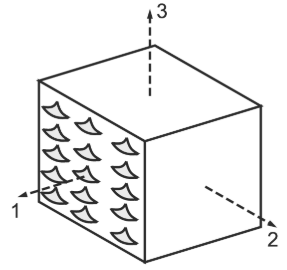
\includegraphics[width=0.25\textwidth]{chapter_2/figures/Principlematerial.PNG}
    \caption{Three principal directions in the axis of asymmetry of a YX[0] produced sample \cite{Rodriguez2001MechanicalInvestigation}}
    \label{fig:Principlematerial}
\end{figure}

If one were to produce test specimens, the convention states that the orientation of the test specimen has two directions which define the orientation of the test specimen, the first being the direction of the longest side of the specimen, the second being the smaller side. In figure \ref{fig:coordinates} the coordinates for sample production are defined. 
To define the direction of the roads (the raster orientation) one could look at the slicer software used (in this case Cura) which defines the deposited road orientation at the angle [0] to be in the Y direction (therefor [90] is in the X direction). Multiple papers use different orientation systems which can be quite confusing and ambiguous. To be consistent and easily comprehensible, this convention will be used throughout this thesis. This will be important when referring to orientations and tested samples in rest of the report. 

After damage or delamination of a layer or a set roads, the properties of the part change, which create a difficult situation to model. H.Li et al. \cite{Li2002CompositeProperties} have developed numerical approaches that uses composite theories including multi-state of elastic, softened and de-bonded state.  Since these are complicated and strongly dependant on the process parameters, these will not be further discussed here. 

%Tanikella, Nagendra G Interesting graph here
%TNO rapport Julius Berens

\section{FFF properties}
    \label{chp:FFF properties}
We have concluded that the process parameters largely influence the properties of FFF produced parts and are dissimilar from conventional produced counterparts. It is made clear that the products from this process create significant anistropy resulting in orthotropic parts (three mutually perpendicular planes of symmetry), porosity, weak layer/road interfaces and surface roughness and inconsistencies. The benefits from FFF produced parts are the geometrical freedom, almost negligible start-up cost due to the absence of a mall or expensive machinery, relatively fast production, integration of different parts without the need of joining and for Defence applications; the large logistic freedom to create parts in remote area's.

\subsection{Experimental mechanical characterization}
Conducting experimental tests with constant process parameters and 100\% infill in the three general directions (as is shown in figure \ref{fig:Principlematerial}) will give more insight in the mechanical behaviour of FFF products. The notation of the produced samples in the 3 directions are respectively; YX[0] direction 1, XY[0] direction 2 and ZY[0] direction 3. The properties that will govern their behaviour will be consecutively; the axial road properties (intra fiber properties), the horizontal (adjacent, inter fiber properties) road bonding, the vertical (stacked, inter fiber properties) layer bonding. This theory is supported by different papers including work done by Alaimo \cite{Alaimo2017InfluenceParts}

Intuitively, the YX[0] specimen would generate the best behaviour, since there are no bonds in the direction of the load. Montero \cite{Montero2001MaterialExperiments} concluded that the bond between layers in shear is stronger and stiffer  than between roads. They also did a tensile test including horizontal specimen with transverse and axially aligned rasters, the results of his stress strain graphs are shown in figure \ref{fig:Transverseraster}. 

\begin{figure}[H]
    \centering
    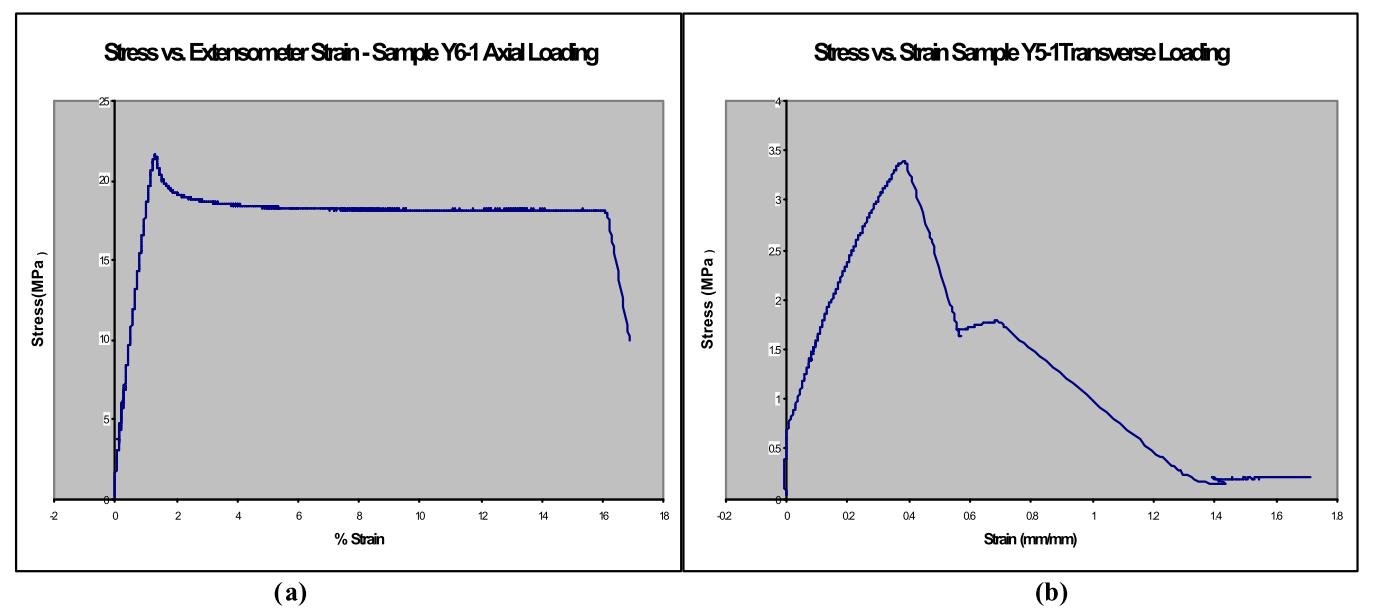
\includegraphics[width=0.8\textwidth]{chapter_2/figures/Transverseraster.PNG}
    \caption{a) (YX)[0] b) (XY)[0] \cite{Montero2001MaterialExperiments}}
    \label{fig:Transverseraster}
\end{figure}

Multiple researchers did similar research, which is limited to the research of the raster orientation in the horizontal plane. This lacks to obtain the information concerning the layer bonding ZY[0]. Rodriguez et al. were probably one of the first to analyze the mechanical behaviour of different FFF orientations, they provide a clear graph (figure \ref{fig:Rodriguezgraph}) comparing the results with bulk ABS \cite{Rodriguez2001MechanicalInvestigation}. This graph clearly suggests an almost linear elastic region with a perfect plastic response for the longitudinal direction and a linear elastic brittle behaviour for the transverse directions. 

\begin{figure}[H]
    \centering
    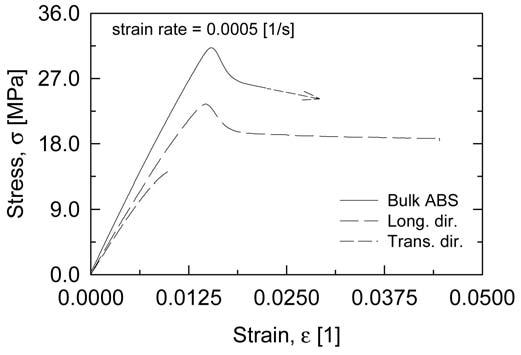
\includegraphics[width=0.5\textwidth]{chapter_2/figures/Rodriguezgraph.jpg}
    \caption{stress strain graph for (YX)[0] (long.dir.) and (XY)[0] \cite{Rodriguez2001MechanicalInvestigation}}
    \label{fig:Rodriguezgraph}
\end{figure}

Without knowing the exact behaviour of the ZY[0] test (3 direction), we can predict (using the properties stated in the TDS of Essentium \cite{EssentiumTechnicalPLA} that it might respond similar to XY[0] but with a lower yield (and UTS) point. However Essentium indicates that the flexural properties of a XY[0] sample are worse than ZY[0]. Montero indicates shear in XY[0] is also worse. Be advised that these experiments are made with different settings and materials, so no conclusions could be made before obtaining comparable data. Blok \cite{Blok2018AnComposites} indicates that the stiffness can be 11\% lower and tensile strength up to 50\% lower in the XY[0] and ZY[0] direction compared wity the YX[0] direction. 

Rodriguez \cite{Rodriguez2001MechanicalInvestigation} also tested the filament and additional features such as crazing and necking. Localized whitening of the specimen has been observed before the yield stress was reached. Failure occurred at whitened areas where localized fiber delamination occurred, these white areas can also be caused by shear bands. He concluded that crazes propagate much faster along the bonding regions than they do in the ABS bulk due to the low interface strength. When loading in the axial direction of the roads there is a small amount of necking observed \cite{Garg2017AnStudy}, which is in line with the stress-strain curve of figure \ref{fig:Rodriguezgraph}. Since crazes are formed due to the plastic deformation induced by polymer stretching, crazing at interroad bonds should suggest a high degree of polymer entanglement.

One of the last things to mention about the result of FFF parts is the assumption of the thermal residual stresses induced by the process. Since they show visco-elastic behaviour at room temperature, one would suggest that the chains would relax over time towards a relaxed state. It has been shown \cite{Veen2019EnhancingTemperature} that thin walled polymer samples with a low $T_g$ will relax its chains after a period of time resulting in a strain in the z direction. %%%%%%%%%%%%%%%%%%extra reference???% 

Annealing and post processing has been discussed to some extent in academic literature (e.g. by Thomas and Rodriguez \cite{Thomas2000ModelingRoads}).

%Constitutive law Domingo, H Li, Bertoldi, Montero, Alaimo, Knoop

%\subsubsection{Road bonding}
%Rodriguez

%(already discussed to some extent)

%\subsubsection{direction}

%Can add math model part of H. Li to thermal analysis and bonding strength
%(already discussed)

%Mechanical behaviour structure, H. Li (very nice paper)

\subsection{Mesostructure}
\label{mesostructure}
The mesostructure of a FFF part (the road structure on 0.1 to 1 millimeter scale) characterizes a significant amount of the mechanical properties of the FFF produced part. It was already discussed that the laminate-like nature of the FFF parts resembles composites. Multiple studies \cite{Somireddy2017MechanicalMesostructure} \cite{Somireddy2018DevelopmentFDM} \cite{Rodriguez2001MechanicalInvestigation} were conducted to characterize the mesostructure by microtoming, a process to cut micrometer thick slices of a specimen, this procedure will be further discussed in chapter 4. Afterwards the sample is inspected with optical microscopy and a digital image is produced. This procedure is used in different scientific fields and has been adopted for the inspection of the cross section of FFF samples. A few, among which Enrique Cuan-Urquizo \cite{Cuan-Urquizo2019CharacterizationApproaches} (\ref{fig:SEMmesostructure}) and Ahn \cite{Ahn2002AnisotropicABS} \ref{fig:AhnMeso}observed the mesostructure (\ref{fig:SEMmesostructure}) with SEM (scanning electron microscope) which gives a more detailed perspective on the mesostructure, but might be too expensive and time-consuming for multiple investigations.

% extra citations \cite{Rodriguez2003MechanicalModeling} \cite{Rodrguez2003DesignStrength} \cite{Sun2008} \cite{Patanwala2018TheComposites} \cite{Li2017TheProperties} \cite{Sheth2017NumericalOrientation} \cite{Li2002CompositeProperties}

The fundamental mesostructure (cross section of XY[0] specimen) is a structured stacking of multiple roads in a rectilinear cadence. If standard extrusion settings are implemented with a well calibrated system, the FFF system should deposit a road structure similar to the one seen in figure \ref{fig:Meso10&20} b. As has been discussed in the section \ref{Process parameters}, the process parameters have a large influence on the result on the mesostructure.  The mesostructure could be optimized (meaning a decrease in porosity) by increasing the flow multiplier.

\begin{figure}[H]
    \centering
    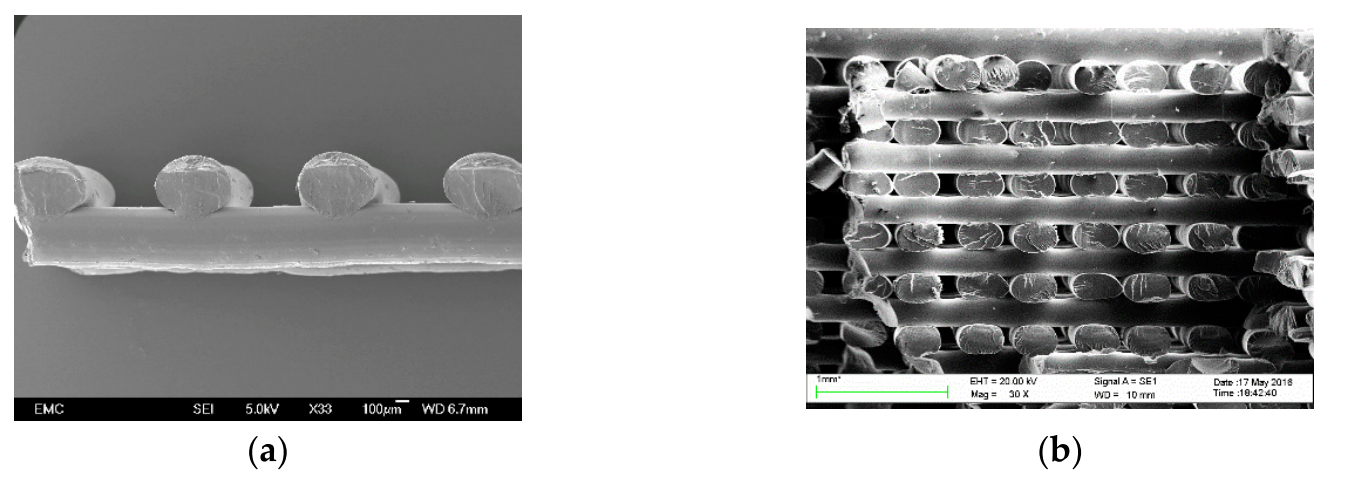
\includegraphics[width=0.5\textwidth]{chapter_2/figures/SEMmesostructure.PNG}
    \caption{Mesostructure observed with SEM by Cuan-Urquizo \cite{Cuan-Urquizo2019CharacterizationApproaches}}
    \label{fig:SEMmesostructure}
\end{figure}

\begin{figure}[H]
    \centering
    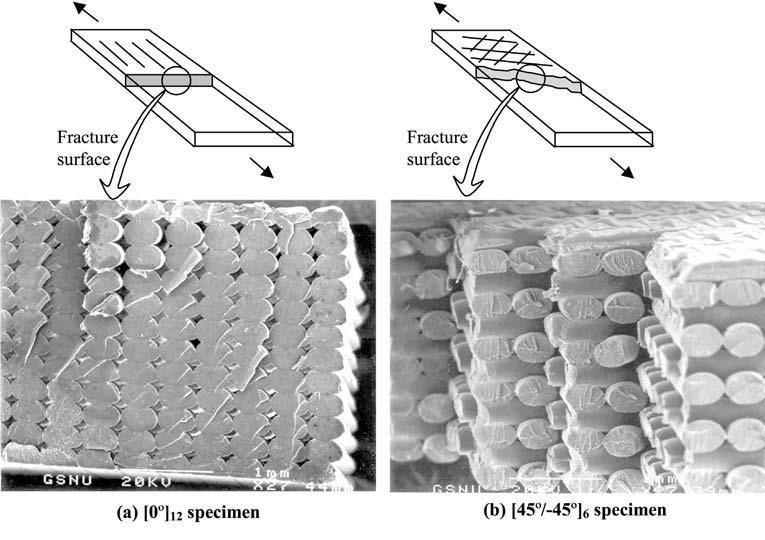
\includegraphics[width=0.5\textwidth]{chapter_2/figures/AhnMeso.jpg}
    \caption{Mesostructure observed with SEM by Ahn \cite{Ahn2002AnisotropicABS}
    \label{fig:AhnMeso}}
\end{figure}

These micrographs give an abundant amount of information on the road structure, wetting, necking and the amount of porosity in a part. This type of characterization is essential to determine the quality of the parts and the consistency of the process. Different systems, parameters and materials have influence on the results of the mesostructure. There is also a common consensus in these studies that the degree of polymer bonding (and consequently weld strength) are a function of the temperature and time of the contact area between two roads. Although, there is not a common agreement on the form of the roads nor the connection to the process parameters and the degree of overlap. The roads are interpreted as different forms by different academici, including ellipses, ovals and oblongs. Someriddy \cite{Somireddy2018DevelopmentFDM} and Sun \cite{Sun2008} assume ellipses in their work, the disadvantage is that the overlapped material is not accounted for. 
It is difficult to make a good assumption concerning the form of the roads in the mesostructure, since the form is largely influenced by the process parameters and other non-controllable process phenomena which  result in a relatively complex form. The reason of characterizing the road form is to be able to model the geometry of the mesostructure in a FEA for the prediction of mechanical properties. This will be further discussed in chapter 5. 
%this is good

%A different approach is followed by the Slic3r manual written by Hodgson \cite{GaryHodgsonSlic3rMath} where he explains how the extruded material of the roads is calculated. In his model he assumes a stadium shaped road, which is also supported by Patanwala \cite{Patanwala2018TheComposites} Additionally to the conclusions found in the section about road width, Hodgson claims that with a higher line width the bonding in the z direction would be better due to a larger contact area and consequently a lower amount of porosity. He explains how the Slic3r software assumes stadium shapes instead of ellipses as is shown in figure \ref{fig:Slic3rshape.png}. 
%The area according to Hodgson is therefore calculated as following: 
%\begin{equation} \label{eqn:crazecriterion}
%A=(w_e-h)\cdoth+\pi(h/2)^2
%\end{equation}
%Where $h$ is the nominal layer height and $w_e$ is the extruded line width. 
%diameter, the excess line width (which was expected to be 10\% by Somireddy) becomes 50\%(!). The micro graphs and single lines produced are in line with the 10\% theory, however the tolerance tests gave results that the parts to be fitted have a over dimension of 0.3-0.4 in 2 directions, resulting in a 75\%-100\% increase in line width, which would actually be closer in line with the Hodgson theory.


%\begin{figure}[H]
    %\centering
    %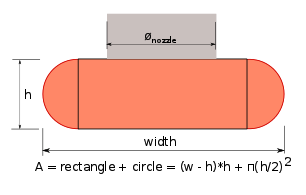
\includegraphics[width=0.5\textwidth]{chapter_2/figures/Slic3rshape.png}
    %\caption{Road shape calculated by the slic3r shoftware \cite{GaryHodgsonSlic3rMath}}
    %\label{fig:Slic3rshape.png}
%\end{figure}

%The ratio between the nominal line width and the nominal layer height is recommended to be around 2, and is not recommended to drop below 1.  
%With this shape a void area is found with this equation:
%\begin{equation}
%A_v = h ^2 - (h/2)^2 \cdot \pi
%\end{equation}
%And the void fraction can be found with
%\begin{equation}
%f_v = \frac{A_v}{A}
%\end{equation}
%He proposes an overlap factor (from 0 to 1) to find the optimum for filling in the void area's, the overlap factor represents how much void remains between the extrusions. It's difficult to estimate this amount, since it also depends on viscosity of plastic, extrusion speed and temperature. To generate enough material to fill in these voids an overlap between two layers should be calculated that encompasses exactly the voids between roads. The equation for the overlap between roads become 
%\begin{equation}
%\delta l = h\cdot (1 - \pi/4)
%\end{equation}
%And additionally,
%\begin{equation}
%w_e = w+\delta l
%\end{equation}

%If considering roads with nominal width of 0.4  and 0.2 heigth, the extrusion width will be 0.44, which is exactly in line with the observations of Somireddy.  

%When creating an alternating raster the mesostructure will obviously be affected. The most common laminates that generate the largest amount of istropy are (YX)[0/90]n and (YX)[45/-45]n, which create laminates that are perpendicular to each other. Hongbin \cite{LiHongbin2017TheProperties} has analysed the (YX)[45/-45]n structure thoroughly. Important to take into account for the prediction of mechanical properties is the different contact areas between layers, since there is no matrix there is a limited contact surface that bonds layers. 

%THINK ABOUT THIS PART
%For regular (YX)[0]n structure the contact area for one road reference to figure \ref{fig:Mesostructurestructure}, is 2x in y direction and 2z in z direction which is continuous in the x direction. 
%%make equation for contact points determined by width and height
%Therefor, if we extrude the road for length w, the contact area of one road would be $((2x)+(2z))\cdot2\cdotw=4(x+z)\cdotw$. However, considering $YX[45/-45]_n$, the contact area of one unit cell of $w\cdoth\cdotw$ would be $(2z)\cdot2\cdotw+2x\cdot2x=4z\cdotw+4x^2$, but since $w>2x$ the resulting contact area will always be smaller than the contact area of $YX[0]_n$.

%A good understanding of the mesostructure can give a better understanding of the mechanical properties of a part when combined with computational models such as Finite Element Analysis (FEA) which could be used to compare the numerical simulation with empirical test to analyze the effect of the polymer orientation on the mechanical properties of a part.

\section{Composite theory}
    \label{Modelling of FFF parts}
Since it was concluded that FFF parts are an-isotropic and have composite like mechanical behaviour due to it's process, it is difficult to predict the properties of such parts. Therefore, it would be beneficial if these properties were possible to model, so the parts could be implemented based on the prediction from the models. 

\subsection{Elastic modelling}
\subsubsection{Stiffness in orthotropic materials}
As has been discussed in the section \ref{chp:FFF properties} we can conclude that the layers are thin and behave as orthotropic material, and therefor, orthotropic constitutive relation for plane stress case can be considered, a similar approach has been found in multiple papers \cite{Rodrguez2003DesignStrength} \cite{Rodriguez2003MechanicalModeling} \cite{Somireddy2018DevelopmentFDM} 
%\cite{Somireddy2017FlexuralStudy} \cite{Somireddy2017MechanicalMesostructure} \cite{Li2017TheProperties} \cite{Ahn2002AnisotropicABS} \cite{Alaimo2017InfluenceParts} \cite{Sheth2017NumericalOrientation} \cite{Patanwala2018TheComposites}. 

The stress strain relation for an orthotropic body can be written in the contracted notation as

\begin{equation}\label{eqn:compliancematrix}
\begin{vmatrix}
\sigma_{11}\\
\sigma_{22}\\
\sigma_{33}\\
\sigma_{12}\\
\sigma_{23}\\
\sigma_{13}\\
\end{vmatrix}
=
\begin{vmatrix}
C_{11}&C_{12}&C_{13}&0&0&0\\
C_{21}&C_{22}&C_{23}&0&0&0\\
C_{31}&C_{32}&C_{33}&0&0&0\\
0&0&0&C_{44}&0&0\\
0&0&0&0&C_{55}&0\\
0&0&0&0&0&C_{66}\\
\end{vmatrix}
\
\begin{vmatrix}
\epsilon_{11}\\
\epsilon_{22}\\
\epsilon_{33}\\
\epsilon_{12}\\
\epsilon_{23}\\
\epsilon_{13}\\
\end{vmatrix}
\end{equation}Since this matrix is diagonally symmetric, the amount of elastic constants is reduced to 9.

Plane stress is achieved by defining $\sigma_{33}$=0 $\sigma_{23}$=0 $\sigma_{13}$=0. The compliance matrix $|C|$ written becomes:


\begin{equation}\label{eqn:compliancematrix}
\begin{vmatrix}
\epsilon_{11}\\
\epsilon_{22}\\
\epsilon_{12}\\
\end{vmatrix}
=
\begin{vmatrix}
\frac{1}{E_1} & \frac{-v_1_2}{E_1} & 0\\
\frac{-v_{12}}{E_1} & \frac{1}{E_2} & 0 \\
0 & 0 & \frac{1}{G_{12}}\\
\end{vmatrix}
\
\begin{vmatrix}
\sigma_{11}\\
\sigma_{22}\\
\sigma_{12}\\
\end{vmatrix}
\end{equation}

The stresses and the stiffness matrix $|Q|$ can be acquired by inverting equation \ref{eqn:compliancematrix} resulting in 

\begin{equation}\label{Stiffnesmatrix}
\begin{vmatrix}
\sigma_{11}\\
\sigma_{22}\\
\sigma_{12}\\
\end{vmatrix}
=
\begin{vmatrix}
\frac{E_1}{1-v_1_2v_2_1} & \frac{-v_1_2E_2}{1-v_1_2v_1_2} & 0\\
\frac{-v_1_2E_2}{1-v_1_2v_1_2} & \frac{E_1}{1-v_1_2v_2_1} & 0 \\
0 & 0 & G_1_2\\
\end{vmatrix}
\
\begin{vmatrix}
\epsilon_{11}\\
\epsilon_{22}\\
\epsilon_{12}\\
\end{vmatrix}
\end{equation}

The resulting independent material constants, $E_1, E_2, v_{12}$ and $G_{12}$ are needed to determine what the mechanical response of a thin FFF product would be.

\subsubsection{Mechanics of Materials}
The mechanics of materials approach is based on simplifying assumptions of either uniform strain or uniform stress in the constituents. These predictions are adequate for longitudinal properties such as Young's modulus $E_1$ and major poisson's ratio $v_{12}$. These properties are not sensitive to fiber shape and distribution, this approach underestimates the transverse and shear properties\cite{Daniel2006EngineeringMaterials}

\subsubsection{Rule of mixtures}
The rule of mixture (ROM) is a commonly used principle in the application of composites, when two different materials are combined in a solid, the ROM can combine the different material properties to predict the new solid characteristics. When loading a composite ply in the 1 direction (along the fibre axis), the elastic properties can be predicted with the parallel or Voigt model\cite{Daniel2006EngineeringMaterials} 

\begin{equation} \label{eqn:Voigt}
E_1=V_f\cdotE_{1f}+(1-V_f)\cdotE_1_m
\end{equation}

Where $E_1$ is the elastic modulus of the ply in direction 1, $V_f$ is the fibre volume and $V_m$ is the matrix volume. Following this formula, and considering the ABS roads as $V_f$ and the porosity as $V_m$, one could predict the elastic properties in the 1 direction by obtaining the void density in the 1 plane.

The different approach can be used for loads in the transverse (2) and (3) directions. The model used for composites is called series of Reuss model \cite{Daniel2006EngineeringMaterials} 

\begin{equation} \label{eqn:Reuss}
E_2=\frac{E_{2f}\cdotE_{2m}}{(E_{2f}\cdotV_m+E_{2m}\cdotV_f)}
\end{equation}
However, this takes a few rough assumptions, since the cross section of the voids are not continuous in the 2 and 3 directions in contrast to the 1 direction, it will be more difficult to determine the void density in the 2 and 3 directions. 

Li et al. \cite{Li2002CompositeProperties} proposes an equation to account for transverse stiffness:

\begin{equation} \label{eqn:ROMseriesfactor}
E_2=\zeta(1-\rho_2)\cdotE
\end{equation}
where $\zeta$ is an empirical factor that takes into account the bonding strength. $\rho_2$ is a linear void fraction along the transverse direction. $1-\rho_2$  represents the relative contact area of the neck between roads. The void area density is determined according to empirical observations. 

Rodriguez \cite{Rodriguez2003MechanicalModeling} proposed a method to obtain the the $E_1$ and $E_2$ where he calculates the cross sectional void density to be squared voids with perfect bonding. He additionally assumes the void density to be uniform in any given plane trough the solid. 
\begin{equation}\label{eqn:E_1}
E_1=(1-\rho_1)\cdotE
\end{equation}The void area density in the 2 direction is assumed to be the square root (one side of the void) of the void area density in the 1 direction.
\begin{equation}\label{eqn:E_2}
E_2=E_3(1-\sqrt{\rho_1})\cdotE
\end{equation}
\subsubsection{Classical Laminate Theory}
It has been made clear that the FFF produced parts have a significant overlap with long fibre composites, due to the linear structure of the road in different layers a FFF produced part can be treated as a laminate with thick fibres and no matrix. The layer can be treated as a lamina or ply, and therefore the classical laminate theory can be employed to account its material behavior in the analysis of the plate. This approach has also been followed by different researchers including Somireddy \cite{Somireddy2018DevelopmentFDM}\cite{Somireddy2017FlexuralStudy}\cite{Somireddy2017MechanicalMesostructure}, Alaimo \cite{Alaimo2017InfluenceParts}, Li \cite{Li2002CompositeProperties} and Casavola \cite{Casavola2016OrthotropicTheory} most of them used it a bases and benchmark for the development of  models to predict the mechanical properties of different ply orientations.

Once the material properties of a single ply are acquired one can predict the properties in different orientations and have them stacked as a composite and predict the properties of the laminate as is shown in figure \ref{fig:Transverseraster}

\begin{figure}[H]
    \centering
    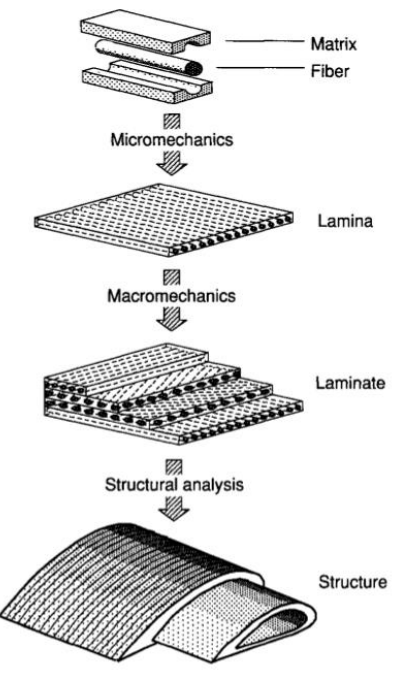
\includegraphics[width=0.25\textwidth]{chapter_2/figures/CompositeTheory.PNG}
    \caption{Principle of the Classical Laminate Theory \cite{Daniel2006EngineeringMaterials}}
    \label{fig:Transverseraster}
\end{figure}
The analytical implementation of the Classical Laminate Theory is widely documented in composite books, and will not be discussed here in further detail. 

\subsubsection{Finite Element Method}    
\label{FiniteElementMethod}
FEM (Finite Element Method), is a popular method to make a structural analysis of a geomtery including constitutive models. The homogenization methods make use of FEM to determine the stresses in the elements in a RVE, this can be applied for composites when combining materials with different properties.

Studies from Garg \cite{Garg2017AnStudy} and Gorski \cite{Gorski2015ComputationMethod}, modeled the road structure in a whole part instead of an RVE. Both Garg \cite{Garg2017AnStudy} and Groski meshed a whole  specimen with roads and performed a FE analyis for different loading conditions. Groski is one of the few that implemented plasticity and failure in his part. He implemented a standard model used by LS-DYNA.  


\subsubsection{Homogenization approach}
%Melro's paper.
An RVE homgogenization approach in combination with the Finite Element Method (implemented with Abaqus software) was proposed by Melro et al. \cite{Melro2012InfluenceMaterials}. A composite consisting of long carbon fibres with an epoxy matrix was modeled on a micro level, with the use of periodic boundary conditions (PBC's), an RVE could be defined to be representative of the bulk properties of the composite. Periodic boundary conditions force such a deformation on the volume element that the displacement of one of the nodes belonging to one edge must be related to the displacement on the corresponding node in the opposite edge\cite{Melro2012InfluenceMaterials}. The volume average of strain in the RVE equals the apllied far-field strain.

\begin{equation}\label{Somireddy2}
\bar{\epsilon}_{ij}=\frac{1}{V_{RVE}}\int_V \epsilon_{ij}dV=\epsilon_{ij}^0
\end{equation}In order to determine the stiffness tensor, where afterwards the 9 elastic constants can be retrieved by inverting the stiffness tensor to the compliance tensor, an analysis for each column should be carried out. Therefore, trough the average volume stress from the elements in the RVE for the 6 different loading conditions the stiffness tensor can be found

\begin{equation}\label{eqn:homogenization}
  \begin{array}{l}
C_{ijkl}=\bar{\sigma}_{ij}=\frac{1}{V_{RVE}}\int_V \sigma_{ij}dV  \\ 

\bar{\epsilon_{kl}}^0=1
\end{array}
\end{equation}

Rodriguez \cite{Rodriguez2003MechanicalModeling} implements a method known as the the asymptotic theory of homogenization. He assumed in his FEM model a mesostructure based on empirically obtained micrographs. This method allowed them to predict the Young's moduli in the 1 and 2 direction with a overestimation of approximately 5 percent.  The reader is referred to his paper for further details.

Apart from Rodriguez, Sheth \cite{Sheth2017NumericalOrientation} has investigated the homogenization method implemented in a damage prediction software, BSAM to predict the elastic properties of the RVE.

Lui and Shapiro \cite{Liu2016HomogenizationStructures} proposed a new approach to find the elastic moduli for the part fabricated by FFF, using Green's function. 

In the homogenization method used in Somireddy's work \cite{Somireddy2018DevelopmentFDM} a RVE is treated as a macroscopically homogeneous orthotropic material. He used a similar method to Melro to homogenize the RVE. Somireddy however, took different sizes of RVE's based on  elliptical road geometry in different directions.

\section{Summary}
From the literature review it is concluded that the process parameters largely influence the properties of FFF products. The three main contributors to the mechanical quality of the part are; the healing and wetting between the roads which is governed by the temperature history in the process; the mesostructure of the cross section which dictates the amount and geometry of porosity. This is mostly influenced by the quality of the process and the printing strategy, and  the properties of the plastic blend that is used. 

Some plastics have have better healing characteristics, this is a matter of the material property called glass transition temperature $T_g$ and the entanglement density $v_e$. Due to the large amount of porosity in samples, the fracture toughness largely dominates the mechanical properties, which in turn is dominated by the entanglement density.

Thermoplastics have complex mechanical behaviour. Since the polymer chains act like in-dependant molecules, the mechanical properties are highly dependant on the temperature and strain rate of the load. There are constitutive models derived from thermosets that predict the yielding, damage and failure of thermoplastics to a certain accuracy. There is some work done on predicting elasticity of FFF products, but very limited results are achieved on non-linear modelling. 

The standardization for production and testing of FFF products is very limited to this day. However, the experimental work done in this field is quite large. The lack of standardization makes it difficult to compare research. 

FFF products exhibit orthotropy, behaving like a laminate of multiple layers. Three principal directions can be distinguished when producing test coupons. The three directions decrease consecutively in mechanical properties. There is no solution yet to increase the isotropy in all directions. 

Micrographs from different studies show significant differences in mesostructure, researchers assume different shapes and models and there is not yet a consensus on the geometry of the mesostructure. 

Since FFF products have large similarities with composites, different analytical and numerical composite theories have been applied successfully to predict the elastic behaviour of FFF products, these include the rule of mixture and the Classical Laminate Theory. There was no successful prediction on non-linear behaviour yet. 


%Homogenization old